%% Bachelor Thesis Template of Xidian Uniersity
%%   for using XDBAthesis package with LaTeX
%%
%% Created by Xue-Jilong(xuejilong@gmail.com)
%%
%% template.tex v0.1, 2011/03/21


\documentclass[xetex,adobefonts,master]{XDBAthesis}
% 选项说明:
% dvipdfm  使用 dvipdfm(x) 生成最终的 PDF 文档 (缺省设置)
% dvips    使用 dvips 生成最终的 PS 文档
% pdftex   使用 pdfLaTeX 生成最终的 PDF 文档
% xetex    使用 XeLaTeX 生成 PD F文档
% adobefonts 使用 Adobe 中文字体
% winfonts 使用 Windows 中文字体
% master   用于生成硕士学位论文

% 图形文件的搜索路径
\graphicspath{{chapter-utf8/}{figures/}}

\begin{document}
%%----------------- 封面部分 ----------------- %%
    \schoolnumber{1203121619}
    \title{基于压缩后缀数组的空间高效}{短读比对算法}   %%题目超过14个字把剩下的放到第二个空
    \entitle{Space-efficient Short Read Alignment with}{ Compressed Suffix Array}   %%题目超过14个字把剩下的放到第二个空
    \major{计算机软件与理论}
    \author{李双江}
    \advisor{霍红卫~~教授}
    \date{2014年11月}
    \majorclass{计算机科学与技术}
    \degreeclass{工科}

    \identifier{10701} %%学校代码
    \classnumber{TP301.6} %%分类好
    \classification{公开}
    \maketitle
    \makethemename
    \makeenthemename
%%----------------- 前言部分 ----------------- %%
    \frontmatter
    \pagestyle{empty}
    \include{chapter-utf8/state}
    \cleardoublepage
\begin{abstract}

新一代基因测序技术(NGS)的出现使得测序成本飞速下降,随之而来的是大量的短读序列
需要更快速准确的比对程序来处理。第一代基于散列表技术的序列比对算法如Bowtie等
能够快速准确的完成比对工作,但其不支持gap比对的特性使得在短读序列(short reads)
过长导致indel出现频繁时,比对的精度也随之下降。另一方面,近年来压缩索引(BWT,CSA,FM-index)
领域的相关研究使得在较小内存中索引人类基因组这样的大规模序列成为可能。这导致
近年来出现了很多基于压缩索引的短读比对算法,如BWA,Bowtie等。本文提出了一种基于压
缩后缀数组和后向搜索实现近似匹配的算法来实现短读比对,在比对时间和空间以及比对
精度上都取得了很好的效果。

基于压缩后缀数组的短读比对算法(CSAA),采用了压缩后缀数组来构建参考序列的索引,
并使用后向搜索来做匹配。通过引入搜索树,CSAA实现了近似匹配算法,从而支持完全的
gap比对。此外CSAA在搜索树上使用了一种类似堆的优先堆数据结构,大大减小了搜索空间。
而且每一次的搜索方向都能保证是最优的。最后结合罚分机制以及$difference$
距离,定义seed等方法,进一步降低搜索空间,提高了CSAA的比对速度和精度。

CSAA的高效体现在三个方面。一是空间高效的索引方法;二是基于后向搜索的高效的近似
匹配方法;三是seed策略和多线程比对技术的利用。本文采用了增量法进行压缩后缀数组索引
的构建,从而跳过后缀数组的构建,降低了对内存的需求。而在比对时,seed的引入使得
在比对短读的前几十个核苷酸就可以放弃大部分无效的搜索方向。多个短读比对的相互
独立使得并行化成为可能,使得CSAA使用多线程时可以获得数倍的加速优势,从而可以根据计算
机的cpu核数指定多个线程,以取得最优的比对速度。


CSAA支持单端和双端序列比对,以Fastq格式输入,输出为标准的SAM(Sequence Alignment Map)
格式。

\keywords{短读比对,序列比对,压缩索引,压缩后缀数组}

\papertype{应用基础研究}

\end{abstract}

\begin{englishabstract}

\setlength\parindent{0em}

\vspace{2ex}
Nowadays,decreasing cost and better accessibility of next generation sequencing methods
have produced a large amount of short reads whic are calling for the development of fast
and accurate read alignment programs.The first generation of hash-table based methods has
been developed,including MAQ,which is accurate,feature rich and fast enough to align short
reads from a single individual.However,Bowtie does not support gapped alignment of longer reads
where indels may occur frequently.On the other hand,recent experimental studies on compressed
index(BWT,CSA,FM-index)have confirmed their practivality for indexing very long strings such
as human genome in the main memory,and many alignment methods based on compressed index have
been developed,for example,BWA.In this paper we show how to build a software called CSAA that
exploits a CSA index of reference sequence,and performs well on alignment speed and accuration.

\vspace{2ex}
We proposed and implemented Compressed Suffix Array Alignment(CSAA),a new short read alignment
tool that is based on backward search with compressed suffix array as index method,to align short reads to a
large reference such as human genome.CSAA uses a search tree on multiple proximate sequences to
support mismatch and gapped alignment,CSAA also introduced a heap like structure to decrease
search space on seach tree.Finally,with the help of penalty strategy and seed,CSAA achieved
similar accuracy and faster speed than MAQ.


\vspace{2ex}
CSAA has three advantages. Firstly,increment CSA construction algorithm has been used in
CSAA,which directly constructs CSA without SA,and uses little memory to classic CSA construction algorithm.
Secondly,CSAA uses seed strategy to speed up alignment,which can drop most of invalid
search direction when aligning the first dozens of nucleotides of a read.Lastly,indpendency of
every short read's aligment makes parallel aligning avaliable.CSAA speed up efficiently by
adopting multi-thread.

\vspace{2ex}
CSAA supports single-end and pair-end mapping with Fastq as input format and SAM(Sequence Alignment Map)
as output format.CSAA also support multi-thread running on a multi-core machine to get a faster
alignment speed.


\englishkeywords{short reads alignment, DNA sequence alignment, compressed index, compressed suffix array}

\papertypeenglish{Applied Basic Research}

\end{englishabstract}


    \listoffigures
    \listoftables
    \begin{symbolstable}\renewcommand{\arraystretch}{1.3}

\noindent
\begin{table}[ht]
\begin{tabular}{p{5cm}p{10cm}}
\textbf{符号}&\textbf{名称}\\
$T$ & 输入的原文本序列串\\
$T[i]$ &输入序列的第$i$个字符\\
$T_i$ &输入序列的第$i$个后缀\\
$P$ & 输入的待查询的序列串\\
$P[i]$ &输入待查训序列的第$i$个字符\\
$n$&输入原串的长度\\
$\Sigma$&字符集\\
$m$ &输入待查训序列的长度\\
$P_i$ &输入待查训序列的第$i$个后缀\\
$l_i$ &模式序列$P_i$在原序列$T$上的位置\\
$\$$ &缀在模式最后的标识字符,小于模式中所有的字符\\
$SA$ &后缀后缀\\
$SA^{-1}$ &后缀数组的逆数组\\
$SA_T$ &输入序列$T$的后缀数组\\
$CSA$ & 压缩后缀数组\\
$\Phi$&压缩后缀数组变换后的数组\\
$difference$ & 短读相似度距离\\
$seed$ & 短读的可信部分\\
\end{tabular}
\end{table}
\noindent
\clearpage
\begin{table}[ht]
\begin{tabular}{p{6.5cm}p{7cm}}
\textbf{函数}&\textbf{名称}\\
$\alpha (c)$ &序列中小于字符$c$的所有字符的个数\\
$\beta (c)$ &序列中等于字符$c$的所有字符的个数\\
$rank_0(i)$ &一个01序列上前$i$位中的所有0的个数\\
$select_0(i)$ &一个01序列上第$i$个0出先的位置\\
$rank_1(i)$ &一个01序列上前$i$位中的所有1的个数\\
$select_1(i)$ &一个01序列上第$i$个1出先的位置\\
$BackwardSearch(P,\Phi,\alpha,\beta)$ & 在压缩后缀数组上用后向搜索方法搜索模式$P$的位置\\
$ExactMatch(c,\Phi,\alpha,\beta,l_{old},r_{old})$& 在压缩后缀数组上做精确匹配$c$\\
$InExactMatch(\Phi,\alpha,\beta,P)$&在压缩后缀数组上做近似匹配$P$\\
$CalculatDifference(\Phi,\alpha,\beta,P)$&计算$P$的$difference$距离\\
$ProcedureIndel(P,\Phi,\alpha,\beta,x,heap)$&处理近似匹配序列$x$的indel\\
$CsaAlignment(\Phi,\alpha,\beta,P)$&在参考序列$T$的压缩后缀数组上比对短读$P$
\end{tabular}
\end{table}

\end{symbolstable}


\begin{abbreviation}\renewcommand{\arraystretch}{1.3}
\noindent
\begin{table}[ht]
\begin{tabular}{p{2cm}p{6cm}p{8cm}}
\textbf{缩略语}&\textbf{英文全称}&\textbf{中文对照}\\
SA &Suffix Array &后缀数组\\
CSA & Compressed Suffix Array &压缩后缀数组\\
CSAA & Compressed Suffix Array shot reads Aligment tool & 压缩后缀数组短读比对工具\\
BWT & Burrows-Wheeler transform&BW变换\\
BWA & BWT short reads Alignment tool & BWT短读比对工具\\
indel & insert and delete &插入和删除\\
\end{tabular}
\end{table}
\end{abbreviation}

    \tableofcontents

%%----------------- 正文部分 ----------------- %%
    \mainmatter
    \pagestyle{content}
    
\chapter{绪论}
\label{chap:introduction}

\section{研究意义和背景介绍}

DNA(脱氧核糖核酸)是生物遗传信息的载体,其双螺旋结构的两个链互相补充,构成稳定结构。其中每个链都含有完备的遗传信息,这些
遗传信息体现在构成DNA链的四种碱基——腺嘌呤(A),胸腺嘧啶(T),鸟嘌呤(C)和胞嘧啶(G)的排列顺序上。在现代生物学研究中,
为分析DNA的遗传表达等特性,需要特定对物种DNA进行测序。早期的sanger测序作为第一代测序手段在人类基因组计划中起到了巨大的作用。

随着生物学,医学等相关科学的发展,新的DNA测序技术不断涌现,其中,以Illumina/Solexa为代表的NGS(NEXT-GENERATION SEQUENCING DAT)
技术以其低廉的测序成本和便捷快速的特点成为当前的主流DNA测序技术。基于这一新技术实现的测序机器每台工作一天就能产生数十亿的
短读序列(short reads)\cite{metzker2009sequencing}。NGS测序技术一般应用于两类测试场景,重测序(Resequencing)
和从头测序(de novo sequencing),这也对应着产生了DNA分析领域的两个最核心的研究问题:比对(alignment)和重组(assembly)。
若测序的目标物种的基因序列之前还从未被测序过,那么从头测序就是研究的第一步,这需要关注把短读以最优方式连接起来。若测序目标
物种已经完成了测序,那么重测序关注的问题是如何把短读序列映射到已知的同物种基因组上,从而分析同源生物的个体基因差异,这个过
程就是本文关注短读比对(short read alignment)。由于每一次测序实验都会得到大量的短读(short reads)序列(5亿到20亿个),同时生物
个体基因之间的差异会导致基因序列存在差异,短读映射面临着基因的近似比对和快速高效比对两个难题。本文即提出一种基于压缩后缀
数组索引算法的快速高效比对算法来解决这两个问题。

重测序得到的短读序列中每一个短读一般不超过1000个碱基(大多数情况下都是20到100个碱基的长度),但一次测序实验中短读数量都
会超过一千万个。参考序列是已经经过准确测序,重组后的已知基因组序列,比如人类基因组序列就是合并出来的总长达2.8G的DNA序列。
出于医疗,身份鉴别等原因会对某个具体的人进行再次DNA测序,这就是DNA重测序,此时测序得到的大量短读序列分析的第一步就是把
这些短读映射到参考序列上,对人类而言,大多都是映射到人类基因组序列上,也可以映射到一个人工合成的参考序列上。映射的过程是
对每一个短读在参考序列上查找的过程,即要在参考序列上找到一个合适的位置,使得从这个位置开始,短读是参考序列的一个子串。

综上所述,短读序列的比对问题可以抽象为一个模式查找问题:给定一个共有$m$个模式的模式集合$P=\{P_1,P_2\ldots P_m\}$,每个
模式的长度已知分别为$l_1,l_2\ldots l_m$,已知一个长为$n$的参考序列$T$,求得一个集合$S=\{s_1,s_2\ldots s_n\}$使
得$P_i=T[s_i\ldots s_i+l_i-1]$。这个查找的过程即为短读到参考序列的比对映射。其中参考序列$T$和短读序列$P_i$都是由DNA测序
中常用的碱基字符$\{A,T,C,G,N\}$构成的。

\section{国内外研究现状}
为实现快速且准确的短读序列映射,近年来出现了很多比对算法。所有这些算法都可以分为两类,一类是通过对短读序列使用散列表等方法建
立短读序列的索引,之后遍历整个参考序列。另一类是为参考序列建立索引,之后再对每个短读进行独立的比对。

第一类比对算法的代表是MAQ,ZOOM,SHRiMP等。MAQ\cite{li2008mapping}基于散列技术,结合短读中每一个核苷酸的测序质量分数,实现了
无空位(ungapped)比对。ZOOM\cite{lin2008zoom}使用了space seeds技术,提高了比对的精确率。而SHRiMP\cite{rumble2009shrimp}则结合space seeds''
和smith-water算法得到了更高的精确率。

第二类算法为参考序列建立索引,通过索引后的数据可以实现快速的比对。如SOAP,WHAM,BFAST等。SOAP\cite{li2008soap}使用seeds技术
和一个散列查询表加速比对,且可以处理较少的空位比对。WHAM\cite{li2012wham}对参考序列建立散列表,先通过散列表查找潜在的比对位置,再进一步比对确定最终结果。BFAST则通过
为参考序列建立多个索引来提高精确度。这几种方法使用的索引方法都需要很大的内存空间,所以比对时空间需求很大,尤其是在用类基因
组这样的较大序列作为参考序列时。在第二类方法中以SOAP2,Bowtie,BWA为代表的基于BW变换(Burrows-Wheeler transform,BWT)\cite{ferragina2005indexing}来创建参考序列
索引的方法具有很大的空间优势。Bowtie\cite{langmead2009ultrafast}使用BWT建立索引,采用回溯递归
的搜索方法,再结合双端搜索实现了高速,空间高效的比对,是目前最快的比对软件之一,但缺陷是不能实现空位(gap)比对。BWA\cite{li2009fast}
也是基于BWT的一种比对算法,比对速度较Bowtie慢,但可实现空位比对。SOAP2\cite{li2009soap2}使用了bidirectional BWT来建立参考序列
的索引,比对速度和Bowtie相当。基于BWT的这些方法都使用了后向搜索方法\cite{lippert2005space}来加速查询。后向搜索可以在$O(m)$时间内实
现长为$m$的字符串的计数查询,以及$O(m\log n)$时间复杂度的query查询。利用后向搜索的性质,Bowtie实现了基于
回溯法的非精确匹配算法,而BWA则采用前缀树搜索的方法实现非精确匹配。在实现非精确匹配的基础上,加上一些打分机制,既实现了短读
序列到参考序列的匹配。

\section{本文的主要内容及组织结构}

本文提出一种采用压缩后缀数组(COmpressed Suffix Array,CSA)建立
索引\cite{grossi2005compressed},实现短读比对的算法:CSAA(csa alienment)。这一算法采用的是CSA的后向搜索特性,同时还使用了
优先队列来保存所有可能的匹配位置,并为每个可能的匹配位置打分,在匹配过程中,通过分支限界抛弃所有低分搜索方向,降低搜索空间,
同时保证匹配结果最优。按照上一节中对短读比对算法的分类,该算法属于对参考序列进行索引的比对算法。


    %%第二章,预备知识
\chapter{预备知识}
\label{chap:predefine}

以BWT为代表的自索引算法近年来在序列比对领域多有出现,例如前文中提到的Bowtie,BWA等。本文提出的序列比对算法使用的也是一种
自索引算法:压缩后缀数组(CSA)\cite{grossi2005compressed}。同BWT相比,CSA的模式查询速度更快,应用于序列比对,相应的比对速
度也会更快,提高整个比对的效率。相应的,在使用CSA之前有必要对CSA的一些概念进行一些简单的叙述,此外序列比对领域的一些基本
概念也会在本章中解释。

\section{压缩后缀数组和模式匹配}

\subsection{后缀数组和压缩后缀数组简介}
压缩后缀数组(CSA)是由Grossi和Vitter\cite{grossi2005compressed}最早提出的第一种实现全文索引的压缩索引数据结构,是对后缀数组(SA)
\cite{manber1993suffix}占用空间过大的改进,并且实现了自索引特性。

设长为$n$的文本序列$T$,字符集为$\Sigma$,本文中将假设$T$有一个特殊的结尾符号$\$$,$\$$不在$\Sigma$中并且字典序小于$\Sigma$
中的所有符号。假设$T$存储在一个数组$T[0\ldots n-1]$中。对任何的整数$i$,假设
\begin{itemize}
    \item $T[i]$为$T$中从左往右0开始的第$i$个字符;
    \item $T_i$为$T$的第$i$个后缀,即$T_i=T[i]T[i+1]\ldots T[n-1]$。
\end{itemize}

$T$的后缀数组$SA[0\ldots n-1]$定义为
$T$的$n$个后缀按字典序排序后的序列,由$\{0,1,\ldots, n-1\}$的一个排列构成,满足$T_{SA[0]}<T_{SA[1]}<\ldots<T_{SA[n-1]}$。即$SA[i]$
表示$T$的$n$个后缀中第$i$小的后缀的开始位置。如表\ref{tab:tabsuffix}所示。后缀数组占用空间$n\log n$,给定文本$T$和其后缀数组
$SA[0\ldots n-1]$,$T$中的任何模式$P$可以在$O(|p|\log n+occ)$时间复杂度内求出其出现位置\cite{manber1993suffix},并且不需要
读原文本$T$。其中$occ$是模式的出现次数。

对于任意的整数$i \in [0\ldots n-1]$,定义$SA^{-1}[i]=j$使得$SA[j]=i$,很明显$SA^{-1}[i]$为$T_i$在$T$的所有后缀中的排名,即
$T$的后缀中比$T_i$小的后缀的数量。

\begin{table}[htbp]
    \caption{$acaaccg\$$的后缀数组和$\Phi$数组}
    \label{tab:tabsuffix}
    \centering
    \begin{tabular}{lllllll}
        \hline\\
        $i$&$T[i]$&$T_i$&$SA[i]$&$T_{SA[i]}$&$\Phi[i]$&$T[SA[i]]$\\
        \hline\\
        0&a&acaaccg\$&7&\$&2&\$\\
        1&c&caaccg\$&2&aaccg\$&3&a\\
        2&a&aaccg\$&0&acaaccg\$&4&a\\
        3&a&accg\$&3&accg\$&5&a\\
        4&c&ccg\$&1&caaccg\$&1&c\\
        5&c&cg\$&4&ccg\$&6&c\\
        6&g&g\$&5&cg\$&7&c\\
        7&a&\$&6&g\$&0&g\\
        \hline
    \end{tabular}
\end{table}

\begin{equation}\label{eq:phi}
    \Phi [i] = j \qquad if\ SA[j] = (SA[i]+1)\mod n \cite{huo2014practical}
\end{equation}

序列 $T$ 的压缩后缀数组(Compressed Suffix Array, CSA)是对后缀数组(SA)空间复杂度过大的一个改进。其本身也是一个包含$n$个
整数与后缀数组$SA$大小相同且由$SA$的近邻函数变换而来的数组$\Phi$。近邻函数定义如\ref{eq:phi},由于$T[n-1]=\$$,所以
$\Phi[0]=SA^{-1}[0]$。另一个角度来看,若后缀$T_k$在$T$的后缀中排名为$i$,则$\Phi[i]$为后缀$T_{k+1}$在$T$的后缀中的排名。
同时,可以看到$SA^{-1}[1]=SA^{-1}[SA[SA^{-1}[0]+1]=\Phi[\Phi[SA[SA^{-1}[0]]]]=\Phi[\Phi[0]]$,同理可以得到$SA^{-1}[2]=\Phi[\Phi[\Phi[0]]]$。
以此类推,即可根据$\Phi[0\ldots n-1]$迭代求出$SA^{-1}[0\ldots n-1]$,由$SA^{-1}[0\ldots n-1]$可快速求出$SA[0\ldots n-1]$。
由此可得出,从后缀数组$SA[0\ldots n-1]$到数组$\Phi[0\ldots n-1]$的变换是可逆的。

$\Phi[0\ldots n-1]$包含$n$个整数,显示存储时,也需要$n\lceil \log n \rceil$位的存储空间,同后缀数组$SA$相同。然而,观察表\ref{tab:tabsuffix}
可以发现$\Sigma[1\ldots n-1]$可以分解为$|\Sigma|$个严格递增的序列,这使得压缩后缀数组可以用简明数据结构存储。而$\Sigma[1\ldots n-1]$
的递增属性则是基于以下引理。

\begin{lem}\label{ref:lem1}
对于任意的整数$i<j$,若$T[SA[i]]=T[SA[j]]$,则$\Phi[i]<\Phi[j]$。
\end{lem}

\begin{proof}
    当$i<j$时,则$T_{SA[i]}<T_{SA[j]}$一定成立,反之亦然。这等价于当$T[SA[i]]=T[SA[j]]$时,$T_{SA[i]+1}<T_{SA[j]+1}$,即$T_{SA[\phi[i]]}<T_{SA[\Phi[j]]}$,
    所以可以得到$\Phi[i]<\Phi[j]$。即引理\ref{ref:lem1}成立。
\end{proof}

对任意一个$\Sigma$中的字符$c$,定义$\alpha(c)$为$T$的后缀中首字符小于$c$的后缀的数目,定义$\beta(c)$为$T$的后缀中首字符为
$c$的后缀的数目。则有以下结论:

\begin{cor}\label{cor1}
对于$\Sigma$中的任意一个字符$c$,$\Phi[\alpha(c)], \Phi[\alpha(c)+1] \ldots \Phi[\alpha(c)+\beta(c)− 1]$是一个严格递增序列。
\end{cor}

\begin{proof}
    对于任意的字符$c$,$T[SA[\alpha(c)]]=T[SA[\alpha(c)+1]]=\ldots =T[SA[\alpha(c)+\beta(c)-1]]=c$,由引理\ref{ref:lem1}可知,
    $\Phi$在$\Phi[\alpha(c)\ldots \alpha(c)+\beta(c)-1]$上严格递增。
\end{proof}

根据以上结论,$\Phi$可以划分为$|\Sigma|$个递增序列,Grossi和Vitter\cite{grossi2005compressed}提出了一种压缩模式来存储$\Phi$,
使得可以在$O(n(H_0+1))$位的空间内存储$\Phi$数组,其中$H_0 \leq \log |\Sigma|$,是文本$T$的0阶经验熵。这种存储模式就是下文中
叙述的简明数据结构。

\subsection{简明数据结构}

简明数据结构(Succint Data Structure)是对整数序列进行简明编码,达到压缩存储的效果并实现常数时间解码的数据结构。本节中将以Vitter
原始论文中的Rice编码为例阐述简明数据结构的存储原理。实际上,除了Rice编码,简明数据结构还可以使用很多编码形式,如$\Delta-\sigma$
编码等。

设有$s$个升序的整数,每一个整数有$w$位,$s<2^w$。简明数据结构的原理是把这$s$个整数分为两部分,分别存储在两个表$Q,R$里。
取出每个整数的前$z=\lfloor \log s\rfloor $位组成一个新的整数,设为$q_i$,明显有$0 \leq q_h \leq q_{h+1} < s$,其中$1 \leq h < s$。
设各个整数中去除前$z$位后剩下的部分组成的整数为$r_1,r_2,\cdots r_s$。

由于$q_1 \leq q_2 \leq \cdots \leq q_s$,所以采用一元编码(unary repesentation)表示$q_i$。对于任意的整数$i \geq 0$,其一元编码为
$0^i1$,即$i$个$0$后紧随一个$1$。在此构建$Q$表采用一元编码表示:$q_1,q_2-q_1,\cdots ,q_s-q_{s-1}$。由此,表$Q$是一个二进制表。加上
辅助数据结构$select$操作,可以在常数时间内获得表$Q$二进制串中第$h$个$1$出现的位置。为获取$q_h$,只需调用$select(h)$获得第$h$个$1$
出现的位置$j$,再通过$j-h$计算出二进制串中前$j$位中$0$的个数,很明显,串中$0$的个数$j-h$即为$q_h$。

表$Q$由两部分组成,表示$q_i$的二进制串和辅助数据结构。总共有$s$个数,所以二进制串中至少有$s$个$1$;$q_i$中最大的数为$2^z$,所以最多
有$2^z$个$0$,所以二进制串的内存空间为$s+2^z \leq 2s$位。而支持$select$操作的辅助数据结构的空间复杂度是$O(s/\log \log s)$ 位,所以$Q$表总的
空间复杂度是$2s+O(s/\log \log n)$。查询时间为常数时间。

对于$R$表,可以简单的当作普通数组存储即可,总共需要$s(w-\lfloor \log s \rfloor)$位,查询时间也为常数时间。

最后,为查询升序整数序列中任意一个整数$s_h$,只需查询$Q$表和$R$表分别获取$q_h$和$r_h$,而后返回$q_h \cdot 2^{w-z}+r_h$即为所查询
的$s_h$。时间复杂度为常数时间。

综上所述,可得以下结论:
\begin{cor}\label{cor2}
对于$s$个升序的整数组成的序列,设每一个整数最多$w$位且$s<2^w$,可以把这$s$个整数存储在最多$s(2+w-\lfloor \log s \rfloor)+O(s/\log \log s)$位
的空间内,且查询任意整数的时间复杂度为$O(1)$。
\end{cor}

\subsection{rank\&select操作}

根据上一小节的论述,简明数据结构实现的基础是rank\&select操作,本节即详细介绍这两个操作的实现方法。Jacobson在论文\cite{jacobson1989space}
中阐述了这两种操作的经典采样分割实现方法。由于经典方法存在空间复杂度较低的问题,本文采用了更高效的RRR方法实现rank\&select操作。

RRR方式是由R.Raman,V.Ramna以及S.Srinivasa Rao等人于2002年提出的一种静态的字典结构\cite{raman2002succinct}。通过这种结构可以
实现对01二元序列的常数时间的rank\&select操作,并且采用同一方法可扩展到对多符号序列的常数时间的rank\&select操作。在二元01序
列上,RRR方法实现rank操作只需要$nH_0 + o(n)$位的空间,而常用的Jacobson的rank\&select方法则需要$n + O(n\log\log n/\log n)$位
的空间\cite{jacobson1989space}。可以看到在01序列中,如果0和1的几率相等时,二者的空间占用相差不大,而若0和1出现的几率并不相
等,其中一个出现的几率远大于另一个时,RRR方法的空间占用将小于n比特。而在压缩后缀数组$\Phi[0\ldots n-1]$的简明存储中,需要维
持一个由01序列构成的采样点的字典结构,该字典需要实现rank\&select操作,且字典中的0远多于1,在这一应用场景中,采用RRR方法要优
于Jacobson的方法。

RRR方法和Jacobson的方法在目录结构上类似,都采用了分块的方法和两层目录结构。具体做法是首先把长为$n$的二元串$B$分长为
$s = \log n^2$的大块$S_1, S_2\ldots S_{n/s}$。之后每一个大块再分成长为$b = \log {n/2}$的小块$B_i(j)$。这两种划分方
法在RRR中和Jacobson的方法是一致的,所不同的是之后的处理。对于每一个小块$B_i(j)$,在Jacobson的方法中是显式直接存储的,
而在RRR方法中则采用了一个$(c, o)$对替代$B_i(j)$,其中$c$表示$B_i(j)$这个小块中的1的个数,即这个小块的类别,而$o$表示$B_i(j)$
在所有的有$c$个1的长为$b$位的证数中的名次。显然,对于第$c$类,总共有$\binom{b}{c}$个。而$c$的最大值为b,所以一个$(c, o)$对
需要的存储空间是$\log{c + 1} + \log{\binom{c}{b}}$位。从这里可以看出,相对于原来的$b$位的原始串,采用一个$(c, o)$对替代后
,所需空间是随原始串中1的个数变化的,1的个数越少(即$c$越小),所需要的存储空间也会相应的变小,而就整体而言,一个$(c, o)$对
所占的空间也是小于$b$位的。这就是RRR方法的优势所在。对于每一类$c$中的每一个$(c, o)$对,都可以预先处理得到这个$(c, o)$对对应
的长为$b$的01串的每一位的$rank$值,并保存为$G_c$表,总共需要$b\log(c + 1)$位的空间。所有的$G_c$表组合起来就构成了我们预处理
得到的表$G$,总共需要$\sum_{c=0}^b {b\log (c+1)\binom{c}{b}=O(\sqrt{n}poly \log n)}$位的空间。

通过上面叙述的方法,可以把每
一个小块$B_i(j)$变换成一个$(c, o)$对,表示为$D_i(j)$,并且$D_i(j)$总共需要$\log(c + 1) + \log\binom{c}{b}$位的空间,累加
所有的小块对应的$(c, o)$对所需要的空间,前面一项累加后为$O(\log\log n)$位,后面一项累加起来为$nH_0$位。把所有的变长的
$D_i(j)$连接起来构成一个单独的表,即$D$表,所需空间为$nH_0 + O(\log\log n)$位。

对于每一个大块$S_i$ ,对应存储一个指针$P_i$指向这个大块的第一个小块对应的$(c, o)$对在$D$表中的位置,即$P_i = D_i(0)$,并
且指针$R_i$存储这个大块对应的第一位的$rank$值,即$R_i = rank((i-1)*s)$。$P$表和$R$表总共需要的空间是$O(n/\log n)$位。同
样的,对应每一个属于大块$S_i$的小块$B_i(j)$,也存储一个指向其$(c, o)$对在$D$表中的位置的指针$L_i(j)$,只是$L_i(j)$是该
位置相对于所在大块位置的相对位置,即$L_i(j) = D_i(j)-P_i$。类似的,保存每一个小块$B_i(j)$的第一位的$rank$值$Q_i(j)$,
当然也是相对于所在大块的$rank$值,即$Q_i(j) = rank((i-1)*s) + (j-1)*b) - R_i$。由于这些相对量的最大值都是$\log n$,所
以$L$表和$Q$表总共需要$O(n \log\log n/\log n)$位的空间。

在求解任意的$rank(p)$时,首先计算第$p$位对应的大块的编号$i = p/s$,
以及小块编号$j = (p -(i -1)*s)/b$,之后,加上所在的大块对应的$rank$值$R_i$和小块对应的相对$rank$值$Q_i(j)$。再根据$P_i$和
$L_i(j)$的值可得到这个小块对应的$(c, o)$对的值$D_i(j)$,通过访问$D$表的$D_i(j)$位置,即可得到第$p$位所在小块的每一位的$rank$
值,加上前面得到的相对$rank$值即可得到最终的$rank$值。

上面所述即为RRR方法的原理,总共需要保存$D,P,R,L,Q$五个表,总的空间需求是$nH_0 + O(n \log\log n/\log n)$位,可以在常数
时间内实现$rank$操作。

RRR方法的$select$操作的实现是基于$rank$的实现的,查找$rank[j]=i$,并且$rank[j-1]=i-1$,则有$select[i]=j$。所以,只需在一直
$rank$时,进行简单的二分查找即可实现求解$select$操作,且不需要任何的额外的辅助空间,时间复杂度是$rank$操作时间复杂度的
$\log n$倍。该方法的优点是实现简单,不需要额外的空间,但却并没有很好的利用RRR方法的性质。从上一小节的叙述中可知,为了实现
RRR的$rank$操作,特意存储了两个目录表,$R$表和$Q$表,其中$R$表是第一级目录,即大块儿的初始位置的$rank$值,而$Q$表是第二级目
录,即各个小块儿的初始位置相对所在大块儿的起始位置的相对$rank$值。利用这一性质,$select$操作可以更高效的完成,原理依然是二
分搜索,但无需对整个序列的$rank$进行二分操作,而是在两层目录上分别进行二分搜索,逐层的缩小搜索的范围,最后实现$select$操作。
具体的计算$select[j]$的算法过程如下:

\begin{algo}
    \qquad \\

    1.首先搜索$R$表,得到一个位置$i$,使得$R[i]<j<R[i+1]$,即可确定$i*s<select[j]<(i+1)*s$。
    
    2.再搜索$Q$表中的$Q[i*s,i*s+1\ldots (i+1)*s]$得到$k$使得$R[i]+Q[k]<j<R[i]+Q[k+1]$ ,即可确定$k*b<j<(k+1)*b$。
    
    3.有了前两部的范围,实际上即得到了对应的第三次查询的需要的大块儿的编号$i$和小块儿的编号$k$,查询$P[i]$和$L[j]$即
    得到了对应的$(c,o)$对在$D$表中的位置,接下来查询$D$表即可得到该$(c,o)$对对应的局部$rank$值。
    
    4.线性查询第3步中得到的$D$表中的$rank$序列,使得$rank[m]=j-R[i]-Q[k]$,则$select[j]=i*s+k*b+m$,即为最终查询结果。
\end{algo}

上述的$select$方法基于二分实现,时间复杂度是三次查询时间复杂度之和,即$\log{n/s}+\log{s/b}+\Theta(b)$。

\section{序列比对}

\subsection{DNA序列格式}

在DNA序列分析领域,DNA数据一般都来自国际知名的几大DNA数据库,如GenBanki,EMBL,DDBJ等。不同的测序方法,通常得到的序列数据也会
有一些差异。对此,为方便后续处理,生物信息学定义了一些通用的序列存储格式,如Fasta,Fastq等。通常Illumina测序数据都是Fastq格式,
所以本文中实现的软件CSAA也以Fastq作为标准输入格式。

Fastq格式是DNA序列格式中常见的一种,Fastq格式的序列一般都包含有四行,第一行由'@'开始,后面跟着序列的描述信息,这点跟Fasta格式
是一样的。第二行是序列的字符表示。第三行由'+'开始,后面也可以跟着序列的描述信息,和第一行信息相同,通常可以省略。第四行是第二行序列的质量评价
(quality values,是测序的质量评价),字符数跟第二行的序列是相等的。下面是Fastq格式序列的一个序列示例。

\begin{verbatim}
@HWUSI-EAS100R:6:73:941:1973#0/1
GATTTGGGGTTCAAAGCAGTATRRRGYKKKMSTCAAATAGTAAATCCATTTGTTCAACT
+HWUSI-EAS100R:6:73:941:1973#0/1
!''*((((***+))%%%++)(%%%%).1***-+*''))**55CCF>>>>>>CCCCCCC6
\end{verbatim}

Illumina测序仪是按照荧光信号来判断所测序的碱基是哪一种的,例如红黄蓝绿分别对应ATCG,但对每个结果都是有一定的误差的。最初sanger
中心用Phred quality score来衡量该read中每个碱基的质量,既$Q=-10\lg P$ ,其中$P$代表该碱基被测序错误的概率,如果该碱基测序
出错的概率为$0.001$,则$Q=30$,30+33=63,63对应的ASCii码为“?”,则在第四行中该碱基对应的质量分数代表值即为“?”。
一般地,碱基质量从0-40,既ASCii码为从 “!”(0+33)到“I”(40+33)。这上是sanger中心采用记录read测序质量的方法,Illumina
没有完全依照sanger中心的方法来定义测序质量,而是把$P$换成了$P/(1-P)$,其他完全按照sanger的定义来做。可以看出当测序质量
很高的情况下两种形式几乎没区别,但低质量的碱基则有区别了。

在Fastq格式中还可能出现其他一些核苷酸符号,具体含义如表\ref{tab:tabatcg}所述。

\begin{table}[htbp]
    \caption{Fastq格式支持的核苷酸符号}
    \label{tab:tabatcg}
    \centering
    \begin{tabular}{ll}
        \hline\\
        核苷酸代码&意义\\
        \hline\\
        A & Adenosine \\
        C & Cytosine \\
        G & Guanine \\
        T & Thymidine \\
        U & Uracil \\
        R & G A (puRine) \\
        Y & T C (pYrimidine) \\
        K & G T (Ketone) \\
        M & A C (aMino group) \\
        S & G C (Strong interaction)\\
        W & A T (Weak interaction) \\
        B & G T C (not A) (B comes after A)\\
        D & G A T (not C) (D comes after C) \\
        H & A C T (not G) (H comes after G) \\
        V & G C A (not T, not U) (V comes after U)\\
        N & A G C T (aNy)\\
        X & masked \\
        - & gap of indeterminate length
    \end{tabular}
\end{table}

DNA序列的标准保存格式是Fastq等格式,同样的,对序列比对的输出格式,也有一个约定的标准数据格式:SAM格式。SAM的全称是
sequence alignment/map format,一般是文本形式的,也可以存为二进制形式文件,即BAM格式。SAM由头文件和map结果组成,头
文件由一行行以“@”起始的注释构成。而map结果是类似下面的文本:

\begin{verbatim}
C12FP66670 0    chr1  12805 1 42M4I5M * 0 0 TTGGATGCCCCTC...
C12FP30032 272  chr1  13494 1 51M     * 0 0 ACTGCCTGGCGCT...
\end{verbatim}

SAM文件中每个read只占一行,被tab分成了很多列,一共有12列,分别记录了:read名称,SAM标记,chromosome名称,5′端起始
位置,MAPQ(mapping quality,描述比对的质量,数字越大,特异性越高),CIGAR字串(记录插入,删除,错配信息),mate名称(
记录mate pair信息),mate的位置,模板的长度,read序列,read质量,程序用标记。

本文中重点关注的是第三列,chrome名称,以及第四列,起始位置。通常作为参考序列的基因组是由多条染色体构成的,比对程序
需要得到read在哪一条染色体上,以及在改染色体上的位置,即5'端起始位置。

\subsection{单端测序和双端测序}
目前的测序方法中,如Solid,都有单端测序(Single-read)和双端测序(Paired end)之分。二者再测序方法上不同,得到的测序数据也有一些
差异。主要区别在于文库的建立上。

无论是单端测序还是双端测序,第一步都是对DNA分子进行切割,这是通过切割酶来实现的。切割后,大DNA分子被切割成长为300bp左右的短
序列(fragments)。测序第二步是增值,通过对这些短序列进行复制,增值,提高DNA分子数量。第三部是加入引物,开始测序。单端测序时
只在DNA短序列分子的一端加上引物,然后依次读取核苷酸,直到读完一个read。通常一个read长为80到1000bp,读取核苷酸时,因为越往后
读取错误率越高,所以一般read序列也是越往后,可靠性越低。双端测序时,会在DNA短序列两端都加上引物,然后分别读取核苷酸。所以,
双端测序得到的是一个DNA短序列分子的两个read,这两个read读取的是DNA链的两个不同的链,并且因为只读取两端的前100bp左右的核苷酸,
所以,这两个read序列并不一定重合,二者之间有一定的距离(distance),distance的长度为短序列(fragment)的长度减去两个短读序列的
长度之和。反映到在参考DNA序列上,distance为两个序列映射位置之差的绝对值。

\section{本章小结}
本章分为两个部分,对本文用到的一些先验知识做了一些简述。第一部分简述了本文要用到的索引算法:压缩后缀数组。描述了其基本特性,
以及可压缩性,接着对简明数据结构做了一些简单介绍,重点是使用到的rank\&select结构:RRR结构。第二部分是对生物信息学领域序列
比对的一些基本概念的解释。包括DNA序列数据格式和单端测序,双端测序的概念。

    \chapter{压缩后缀数组的实现}

\section{后缀数组和压缩后缀数组}
压缩后缀数组(CSA)是由Grossi和Vitter\cite{grossi2005compressed}最早提出的第一种实现全文索引的压缩索引数据结构,是对后缀数组(SA)
\cite{manber1993suffix}占用空间过大的改进,并且实现了自索引特性。

设长为$n$的文本序列$T$,字符集为$\Sigma$,本文中将假设$T$有一个特殊的结尾符号$\$$,$\$$不在$\Sigma$中并且字典序小于$\Sigma$
中的所有符号。假设$T$存储在一个数组$T[0\ldots n-1]$中。对任何的整数$i$,假设
\begin{itemize}
    \item $T[i]$为$T$中从左往右0开始的第$i$个字符;
    \item $T_i$为$T$的第$i$个后缀,即$T_i=T[i]T[i+1]\ldots T[n-1]$。
\end{itemize}

$T$的后缀数组$SA[0\ldots n-1]$定义为
$T$的$n$个后缀按字典序排序后的序列,由$\{0,1,\ldots, n-1\}$的一个排列构成,满足$T_{SA[0]}<T_{SA[1]}<\ldots<T_{SA[n-1]}$。即$SA[i]$
表示$T$的$n$个后缀中第$i$小的后缀的开始位置。如表\ref{tab:tabsuffix}所示。后缀数组占用空间$n\log n$,给定文本$T$和其后缀数组
$SA[0\ldots n-1]$,$T$中的任何模式$P$可以在$O(|p|\log n+occ)$时间复杂度内求出其出现位置\cite{manber1993suffix},并且不需要
读原文本$T$。其中$occ$是模式的出现次数。

对于任意的整数$i \in [0\ldots n-1]$,定义$SA^{-1}[i]=j$使得$SA[j]=i$,很明显$SA^{-1}[i]$为$T_i$在$T$的所有后缀中的排名,即
$T$的后缀中比$T_i$小的后缀的数量。

\begin{table}[htbp]
    \caption{$acaaccg\$$的后缀数组和$\Phi$数组}
    \label{tab:tabsuffix}
    \centering
    \begin{tabular}{lllllll}
%        \hline\\
        \toprule
        $i$&$T[i]$&$T_i$&$SA[i]$&$T_{SA[i]}$&$\Phi[i]$&$T[SA[i]]$\\
%        \hline\\
        \midrule
        0&a&acaaccg\$&7&\$&2&\$\\
        1&c&caaccg\$&2&aaccg\$&3&a\\
        2&a&aaccg\$&0&acaaccg\$&4&a\\
        3&a&accg\$&3&accg\$&5&a\\
        4&c&ccg\$&1&caaccg\$&1&c\\
        5&c&cg\$&4&ccg\$&6&c\\
        6&g&g\$&5&cg\$&7&c\\
        7&a&\$&6&g\$&0&g\\
%        \hline
        \bottomrule
    \end{tabular}
\end{table}

\begin{equation}\label{eq:phi}
    \Phi [i] = j \qquad if\ SA[j] = (SA[i]+1)\mod n \cite{huo2014practical}
\end{equation}

序列 $T$ 的压缩后缀数组(Compressed Suffix Array, CSA)是对后缀数组(SA)空间复杂度过大的一个改进。其本身也是一个包含$n$个
整数与后缀数组$SA$大小相同且由$SA$的近邻函数变换而来的数组$\Phi$。近邻函数定义如\ref{eq:phi},由于$T[n-1]=\$$,所以
$\Phi[0]=SA^{-1}[0]$。另一个角度来看,若后缀$T_k$在$T$的后缀中排名为$i$,则$\Phi[i]$为后缀$T_{k+1}$在$T$的后缀中的排名。
同时,可以看到$SA^{-1}[1]=SA^{-1}[SA[SA^{-1}[0]+1]=\Phi[\Phi[SA[SA^{-1}[0]]]]=\Phi[\Phi[0]]$,同理可以得到$SA^{-1}[2]=\Phi[\Phi[\Phi[0]]]$。
以此类推,即可根据$\Phi[0\ldots n-1]$迭代求出$SA^{-1}[0\ldots n-1]$,由$SA^{-1}[0\ldots n-1]$可快速求出$SA[0\ldots n-1]$。
由此可得出,从后缀数组$SA[0\ldots n-1]$到数组$\Phi[0\ldots n-1]$的变换是可逆的。

$\Phi[0\ldots n-1]$包含$n$个整数,显示存储时,也需要$n\lceil \log n \rceil$位的存储空间,同后缀数组$SA$相同。然而,观察表\ref{tab:tabsuffix}
可以发现$\Sigma[1\ldots n-1]$可以分解为$|\Sigma|$个严格递增的序列,这使得压缩后缀数组可以用简明数据结构存储。而$\Sigma[1\ldots n-1]$
的递增属性则是基于以下引理。

\begin{lem}\label{ref:lem1}
对于任意的整数$i<j$,若$T[SA[i]]=T[SA[j]]$,则$\Phi[i]<\Phi[j]$。
\end{lem}

\begin{proof}
    当$i<j$时,则$T_{SA[i]}<T_{SA[j]}$一定成立,反之亦然。这等价于当$T[SA[i]]=T[SA[j]]$时,$T_{SA[i]+1}<T_{SA[j]+1}$,即$T_{SA[\phi[i]]}<T_{SA[\Phi[j]]}$,
    所以可以得到$\Phi[i]<\Phi[j]$。即引理\ref{ref:lem1}成立。
\end{proof}

对任意一个$\Sigma$中的字符$c$,定义$\alpha(c)$为$T$的后缀中首字符小于$c$的后缀的数目,定义$\beta(c)$为$T$的后缀中首字符为
$c$的后缀的数目。则有以下结论:

\begin{cor}\label{cor1}
对于$\Sigma$中的任意一个字符$c$,$\Phi[\alpha(c)], \Phi[\alpha(c)+1] \ldots \Phi[\alpha(c)+\beta(c)− 1]$是一个严格递增序列。
\end{cor}

\begin{proof}
    对于任意的字符$c$,$T[SA[\alpha(c)]]=T[SA[\alpha(c)+1]]=\ldots =T[SA[\alpha(c)+\beta(c)-1]]=c$,由引理\ref{ref:lem1}可知,
    $\Phi$在$\Phi[\alpha(c)\ldots \alpha(c)+\beta(c)-1]$上严格递增。
\end{proof}

根据以上结论,$\Phi$可以划分为$|\Sigma|$个递增序列,这个递增性质是压缩后缀数组可压缩性的本质保证。Grossi和Vitter\cite{grossi2005compressed}
据此提出了一种压缩模式来存储$\Phi$,使得可以在$O(n(H_0+1))$位的空间内存储$\Phi$数组,其中$H_0 \leq \log |\Sigma|$,是文
本$T$的0阶经验熵。这种存储模式就是下文中所叙述的简明数据结构。

\section{简明数据结构}

简明数据结构(Succint Data Structure)\cite{jacobson1988succinct}是对整数序列进行简明编码,达到压缩存储的效果并实现常数时间解码的一类数据结构的总称。本节中
将以Vitter原始论文中使用的Rice编码为例阐述简明数据结构的存储原理。实际上,除了Rice编码,简明数据结构还可以使用很多编码形式,
如Elias编码\cite{witten1999managing}等。

在介绍简明数据结构之前,我们需要先定义$rank\&select$两个操作。

\begin{defn}\label{def:rank}
在一个01二元序列$B$上,$rank_0(i)$操作定义为$B$表中前$i$位中0的个数;而$select_0(i)$定义为$B$表中第$i$个0的下标位置。类似的
$rank_1(i)$和$select_1(i)$则定义为$B$表中前$i$位中1的个数,和第$i$个1在$B$表中的下标。
\end{defn}

设有$s$个升序的整数,每一个整数有$w$位,$s<2^w$。简明数据结构的原理是把这$s$个整数分为两部分,分别存储在两个表$Q,R$里。
取出每个整数的前$z=\lfloor \log s\rfloor $位组成一个新的整数,设为$q_i$,明显有$0 \leq q_h \leq q_{h+1} < s$,其中$1 \leq h < s$。
设各个整数中去除前$z$位后剩下的部分组成的整数为$r_1,r_2,\cdots r_s$。

由于$q_1 \leq q_2 \leq \cdots \leq q_s$,所以采用一元编码(unary repesentation)表示$q_i$。对于任意的整数$i \geq 0$,其一元编码为
$0^i1$,即$i$个$0$后紧随一个$1$。在此构建$Q$表采用一元编码表示:$q_1,q_2-q_1,\cdots ,q_s-q_{s-1}$。由此,表$Q$是一个二进制表。加上
辅助数据结构$select$操作,可以在常数时间内获得表$Q$二进制串中第$h$个$1$出现的位置。为获取$q_h$,只需调用$select(h)$获得第$h$个$1$
出现的位置$j$,再通过$j-h$计算出二进制串中前$j$位中$0$的个数,很明显,串中$0$的个数$j-h$即为$q_h$。

表$Q$由两部分组成,表示$q_i$的二进制串和辅助数据结构。总共有$s$个数,所以二进制串中至少有$s$个$1$;$q_i$中最大的数为$2^z$,所以最多
有$2^z$个$0$,所以二进制串的内存空间为$s+2^z \leq 2s$位。而支持$select$操作的辅助数据结构的空间复杂度是$O(s/\log \log s)$ 位,所以$Q$表总的
空间复杂度是$2s+O(s/\log \log n)$。查询时间为常数时间。

对于$R$表,可以简单的当作普通数组存储即可,总共需要$s(w-\lfloor \log s \rfloor)$位,查询时间也为常数时间。

最后,为查询升序整数序列中任意一个整数$s_h$,只需查询$Q$表和$R$表分别获取$q_h$和$r_h$,而后返回$q_h \cdot 2^{w-z}+r_h$即为所查询
的$s_h$。时间复杂度为常数时间。

综上所述,可得以下结论:
\begin{cor}\label{cor2}
对于$s$个升序的整数组成的序列,设每一个整数最多$w$位且$s<2^w$,使用Rice编码,可以把这$s$个整数存储在最多$s(2+w-\lfloor \log s \rfloor)+O(s/\log \log s)$位
的空间内,且查询任意整数的时间复杂度为$O(1)$。
\end{cor}

以上是使用Rice编码$\Phi[0\ldots n-1]$,若使用Elias delta编码,压缩效率会更高。假设一个整数$p$的二进制表示为$b(p)$,那么$p$的
Elias delta编码为$1^{|b(r)|}0b(r)b(p)$,这里$r=|b(p)|$是$p$的二进制表示的位数。该编码的长度是$\log (2\log p +1)+1+\log p =\log p(1+o(1))$。
对于$\Phi[\alpha(c),\alpha(c)+1\ldots \alpha(c)+\beta(c)-1]$,因为是一个递增序列,所以对其前后差值编码。所以对于$\Phi$的一个递增区间,
用alias delta编码的总长度为$\sum_{i,i-1 \in \{\alpha(c),\alpha(c)+1 \ldots \alpha(c)+\beta(c)-1\}} (1+o(1))\log(\Phi[i]-\Phi[i-1])$位。
这在最坏情况下为$\beta(c)(1+o(1))\log(n/\beta(c))$。因此整个$\Phi[0\ldots n-1]$用Alisa delta编码的总长度为:
\begin{equation}
\sum_{c \in \Sigma} \beta(c)(1+o(1))\log(n/\beta(c))=nH_0(1+o(1))
\end{equation}

现在考虑如何解码Elias delta编码,如上文所示,首先需要找到第一个0的位置,并计算0之前1的个数。这一步操作可以使用$rank\&select$操作
在常数时间内完成,即先解码$1^{|b(r)|}0$,得到$|b(r)|=select_0(1)$,再解码$b(r)$,最后得到$b(p)$,完成解码。对应到CSA的$\Phi$数组
上,因为是差分存储,所以需要逐步解码$\Phi$,在实际应用中可以分块采样加速解码$\Phi$。

综上两种简明数据结构,要实现对$\Phi$数组的压缩存储的基础都是$rank\&select$操作。下一小节对$rank\&select$操作给出详细介绍。

\section{rank\&select操作}

根据上一小节的论述,简明数据结构实现的基础是$rank\&select$操作,本节即详细介绍这两个操作的实现方法。Jacobson在论文\cite{jacobson1989space}
中阐述了这两种操作的经典采样分割实现方法。由于经典方法存在空间复杂度较低的问题,本文采用了更高效的RRR方法实现rank\&select操作。

RRR方式是由R.Raman,V.Ramna以及S.Srinivasa Rao等人于2002年提出的一种静态的字典结构\cite{raman2002succinct}。通过这种结构可以
实现对01二元序列的常数时间的rank\&select操作,并且采用同一方法可扩展到对多符号序列的常数时间的rank\&select操作。在二元01序
列上,RRR方法实现rank操作只需要$nH_0 + o(n)$位的空间,而常用的Jacobson的rank\&select方法则需要$n + O(n\log\log n/\log n)$位
的空间\cite{jacobson1989space}。可以看到在01序列中,如果0和1的几率相等时,二者的空间占用相差不大,而若0和1出现的几率并不相
等,其中一个出现的几率远大于另一个时,RRR方法的空间占用将小于n比特。而在压缩后缀数组$\Phi[0\ldots n-1]$的简明存储中,需要维
持一个由01序列构成的采样点的字典结构,该字典需要实现rank\&select操作,且字典中的0远多于1,在这一应用场景中,采用RRR方法要优
于Jacobson的方法。

\subsection{RRR方法的理论基础}\label{chap:sub1}
RRR方法和Jacobson的方法在目录结构上类似,都采用了分块的方法和两层目录结构。具体做法是首先把长为$n$的二元串$B$分长为
$s = \log n^2$的大块$S_1, S_2\ldots S_{n/s}$。之后每一个大块再分成长为$b = \log {n/2}$的小块$B_i(j)$。这两种划分方
法在RRR中和Jacobson的方法是一致的,所不同的是之后的处理。对于每一个小块$B_i(j)$,在Jacobson的方法中是显式直接存储的,
而在RRR方法中则采用了一个$(c, o)$对替代$B_i(j)$,其中$c$表示$B_i(j)$这个小块中的1的个数,即这个小块的类别,而$o$表示$B_i(j)$
在所有的有$c$个1的长为$b$位的证数中的名次。显然,对于第$c$类,总共有$\binom{b}{c}$个。而$c$的最大值为b,所以一个$(c, o)$对
需要的存储空间是$\log{c + 1} + \log{\binom{c}{b}}$位。从这里可以看出,相对于原来的$b$位的原始串,采用一个$(c, o)$对替代后
,所需空间是随原始串中1的个数变化的,1的个数越少(即$c$越小),所需要的存储空间也会相应的变小,而就整体而言,一个$(c, o)$对
所占的空间也是小于$b$位的。这就是RRR方法的优势所在。对于每一类$c$中的每一个$(c, o)$对,都可以预先处理得到这个$(c, o)$对对应
的长为$b$的01串的每一位的$rank$值,并保存为$G_c$表,总共需要$b\log(c + 1)$位的空间。所有的$G_c$表组合起来就构成了我们预处理
得到的表$G$,总共需要$\sum_{c=0}^b {b\log (c+1)\binom{c}{b}=O(\sqrt{n}poly \log n)}$位的空间。

通过上面叙述的方法,可以把每
一个小块$B_i(j)$变换成一个$(c, o)$对,表示为$D_i(j)$,并且$D_i(j)$总共需要$\log(c + 1) + \log\binom{c}{b}$位的空间,累加
所有的小块对应的$(c, o)$对所需要的空间,前面一项累加后为$O(\log\log n)$位,后面一项累加起来为$nH_0$位。把所有的变长的
$D_i(j)$连接起来构成一个单独的表,即$D$表,所需空间为$nH_0 + O(\log\log n)$位。

对于每一个大块$S_i$ ,对应存储一个指针$P_i$指向这个大块的第一个小块对应的$(c, o)$对在$D$表中的位置,即$P_i = D_i(0)$,并
且指针$R_i$存储这个大块对应的第一位的$rank$值,即$R_i = rank((i-1)*s)$。$P$表和$R$表总共需要的空间是$O(n/\log n)$位。同
样的,对应每一个属于大块$S_i$的小块$B_i(j)$,也存储一个指向其$(c, o)$对在$D$表中的位置的指针$L_i(j)$,只是$L_i(j)$是该
位置相对于所在大块位置的相对位置,即$L_i(j) = D_i(j)-P_i$。类似的,保存每一个小块$B_i(j)$的第一位的$rank$值$Q_i(j)$,
当然也是相对于所在大块的$rank$值,即$Q_i(j) = rank((i-1)*s) + (j-1)*b) - R_i$。由于这些相对量的最大值都是$\log n$,所
以$L$表和$Q$表总共需要$O(n \log\log n/\log n)$位的空间。

在求解任意的$rank(p)$时,首先计算第$p$位对应的大块的编号$i = p/s$,
以及小块编号$j = (p -(i -1)*s)/b$,之后,加上所在的大块对应的$rank$值$R_i$和小块对应的相对$rank$值$Q_i(j)$。再根据$P_i$和
$L_i(j)$的值可得到这个小块对应的$(c, o)$对的值$D_i(j)$,通过访问$D$表的$D_i(j)$位置,即可得到第$p$位所在小块的每一位的$rank$
值,加上前面得到的相对$rank$值即可得到最终的$rank$值。

上面所述即为RRR方法的原理,总共需要保存$D,P,R,L,Q$五个表,总的空间需求是$nH_0 + O(n \log\log n/\log n)$位,可以在常数
时间内实现$rank$操作\cite{makinen2007implicit}。

RRR方法的$select$操作的实现是基于$rank$的实现的,查找$rank[j]=i$,并且$rank[j-1]=i-1$,则有$select[i]=j$。所以,只需在一直
$rank$时,进行简单的二分查找即可实现求解$select$操作,且不需要任何的额外的辅助空间,时间复杂度是$rank$操作时间复杂度的
$\log n$倍。该方法的优点是实现简单,不需要额外的空间,但却并没有很好的利用RRR方法的性质。从上一小节的叙述中可知,为了实现
RRR的$rank$操作,特意存储了两个目录表,$R$表和$Q$表,其中$R$表是第一级目录,即大块儿的初始位置的$rank$值,而$Q$表是第二级目
录,即各个小块儿的初始位置相对所在大块儿的起始位置的相对$rank$值。利用这一性质,$select$操作可以更高效的完成,原理依然是二
分搜索,但无需对整个序列的$rank$进行二分操作,而是在两层目录上分别进行二分搜索,逐层的缩小搜索的范围,最后实现$select$操作。
具体的计算$select[j]$的算法过程如下:
\begin{algorithm}
    \caption{RRR select(j)算法}
    \label{alg:rrrselect}
    \begin{algorithmic}[1]
        \Require $R,Q,P,L,D,s,j$
        \Ensure $select(j)$
        \State 首先搜索$R$表,得到一个位置$i$,使得$R[i]<j<R[i+1]$,即可确定$i*s<select[j]<(i+1)*s$。
        \State 再搜索$Q$表中的$Q[i*s,i*s+1\ldots (i+1)*s]$得到$k$使得$R[i]+Q[k]<j<R[i]+Q[k+1]$ ,即可确定$k*b<j<(k+1)*b$。
        \State 有了前两部的范围,实际上即得到了对应的第三次查询的需要的大块儿的编号$i$和小块儿的编号$k$,查询$P[i]$和$L[j]$即
               得到了对应的$(c,o)$对在$D$表中的位置,接下来查询$D$表即可得到该$(c,o)$对对应的局部$rank$值。 
        \State 线性查询第3步中得到的$D$表中的$rank$序列,使得$rank[m]=j-R[i]-Q[k]$,则$select[j]=i*s+k*b+m$,即为最终查询结果。
    \end{algorithmic}
\end{algorithm}

上述的$select$方法基于二分实现,时间复杂度是三次查询时间复杂度之和,即$\log{n/s}+\log{s/b}+\Theta(b)$。

\subsection{RRR方法的实现}

上一小结介绍了RRR的理论实现方法,这种方法有比较好的理论基础,但实际上过于复杂,并不适合具体的实现。两层目录,四个表最终
在实际环境中所占的空间会很大,空间效率并不是很具优势。故在实际应用实现中一般会做一些简化处理,从而得到更好的空间效率。下
面论述的既是一种高效的具有实际应用效果的实现方法。

首先,不同于理论中需要随输入数据规模可变的块长,实现时只要一层目录,且把小块的长度$b$固定为15,这样每一个$c$都恰好只需
一个4位的整数来表示,$o$的保存方法不变,对于$D$表,只需要把所有的15位的整数重新按类别$c$排序,同一类的数放在一个桶内,
所有的桶链接成一个表,这个表实际上存储了215个16位的整数,总共只需要64KB的空间。$D$表放弃了保存每一个$b$位长的整数的
每一个$rank$值,这导致最终需要平均4次操作才能得到任意一个位的$rank$,相对于原始论文中的方法,时间效率有所下降。但空间
效率得到了改善。同样的为了减少空间占用,我们把两层目录改为单层目录,每一个大块的长度可为15的整数倍$k$,即每一个大块
中包含$k$个小块,对每一个小块保存两个表,$R$和$S$。其中$R$表保存每一个小块的类别$c$,即这个小块有多少个1;$S$表保存每
一个小块对应的$o$值,即这个小块在所述类别中的位置。明显的$R$表总共需要$4n/15 = 0.25n$位的空间,而$S$表总共需要
$\log(\frac{15}{c_1})+\log(\frac{15}{c_2})+\ldots+\log(\frac{15}{c_{n/15}})$位。有了$R$和$S$表,只需顺序访问$R$表即可
得到对应小块对应的$c$,经过累加计算访问$S$表可得到$o$,再根据$(c, o)$对访问$D$表即可得到对应小块的真实01序列。但要求得
任意位置的$rank$值,则还需加上两个辅助结构,$sumR$和$sumS$表。其中$sumR[i]$保存的是第$i$个大块的第一位所在位置的$rank$
值,即$sumR[i] = rank(i⋅15⋅k − 1)$,$S$表保存每一个大块的第一个小块对应的$(c, o)$对的$o$值所在在$S$表中的偏移量。


对于要解码的任意的$rank[p]$,首先计算其所在大块的编号$i = p/(k⋅15)$,再计算其所在小块的编号$j = p/15$。之后我们即可计
算出$p$所在小块的第一位的$rank$值为$sumR[i]+\sum_{t=i*k}^{j-1}R[t]$,其中$R[t]$为第$t$个小块对应的$c$值,这个值可以在
$R$表上常数时间内得到。有了这个相对值,借助于$sumS[i]+ \sum_{t=i*k}^{j-1}(\frac{b}{R[t]})$即可得到对应小块的$o$值在$S$
表上的偏移量,访问$S$表即可得到$o$值,接着利用得到的$(c, o)$对去访问$D$表就可以得到这个小块的原始01序列,再借助$popcount$
指令,可以在常数时间内获得这个小块内任意位置的$rank$值,和之前的相对$rank$值相加即为最终的$rank$值。总的时间开销会大于
Jacobson的方法,比原始$RRR$论文中的方法也稍慢,但总的空间效率则得到了极大的提高。

对应于$rank$的实现方法,$select$的实现方法也要和理论方法稍有不同。但本质的方法是相同的,依然是在每一层上进行二分搜索。具体
的求解$select[j]$的算法如下:
\begin{algorithm}
    \caption{select实现}
    \begin{algorithmic}[1]
        \Require $sumR,R,,sumS,D,j$
        \Ensure $select(j)$
        \State 首先在$sumR$表上二分搜索$i$,使得$sumR[i]<j<sumR[i+1]$,则可以判定$i*15<select[j]<(i+1)*15$。
        \State 接着在$R$表的$R[i*15\ldots i*(15+1)]$上线性搜索,使得$sumR[i]+\sum_{t=i*15}^k R[t]<j< sumR[i]+\sum_{t=i*15}^{k+1}R[t]$。
    此时可以判定$k*15<select[j]<(k+1)*15$。
        \State 接着需要根据$R[k]$和$sumS[i]+\sum_{t=i*15}^{k-1}(\frac{b}{R[t]})$得到对应的$(c,o)$对,从而查询$D$表得到对应的15位01串。
        \State 根据3中得到的01串,线性搜索这个01串,使得$sumR[i]+\sum_{t=i*15}{k}R[t]+P(m)=j$,其中$P(m)$为3中所得01串上前$m$
    位的$popCount$值,则可得最终的结果为$select(j)=k*15+m$
    \end{algorithmic}
\end{algorithm}

由上述算法描述可以看到,$select$的实现是在1次二分搜索和若干次线性搜索的基础上完成的。总的时间复杂读是三次搜索时间复杂度之和,即:
$\log (\frac{n}{15*k}) +\Theta(k)+O(1)$,其中$k$为整数,意义是每一个大块儿中所包含的小块儿的数目。

\subsection{RRR方法实验结果}
综上所述,可以看出RRR方法空间效率是其优势所在,所以这一小节,我们通过实验着重测试RRR方法的空间占用,并且和Jacobson的方法在同一
测试平台上进行实验结果对比。测试数据是随机构造的01序列,其中1的出现几率为10\%。数据的规模是64M到1G的01序列。测试环境是在普通
PC机上,拥有4G的内存和双核奔腾CPU。结果如表\ref{tab:tabrrr}所示,而Jacobson的方法在同样测试条件下的效果在表\ref{tab:tabjacobson}。

\begin{table}[htbp]
    \caption{RRR方法的时间效率和空间效率}
    \label{tab:tabrrr}
    \centering
    \begin{tabularx}{1.0\textwidth}{lXlll}
        \toprule
        数据规模(MB)&rank\&select结构大小(Byte)&Bit Per Symbol&rank时间(us)&get时间(us)\\
        \midrule
        64&5557352&0.6625&1.46&1.46\\
        128&11064000&0.6595&1.47&1.45\\
        256&22092224&0.6584&1.47&1.46\\
        512&44178496&0.6583&1.52&1.46\\
        1024&88410688&0.6583&1.52&1.46\\
        \bottomrule
    \end{tabularx}
\end{table}

\begin{table}[htbp]
    \caption{Jacobson方法的时间效率和空间效率}
    \label{tab:tabjacobson}
    \centering
    \begin{tabularx}{1.0\textwidth}{lXlll}
        \toprule
        数据规模(MB)&rank\&select结构大小(Byte)&Bit Per Symbol&rank时间(us)&get时间(us)\\
        \midrule
        64&1.927e+7&2.297&0.536&0\\
        128&3.6148e+7&2.297&0.536&0\\
        256&7.22991e+7&2.1546&0.543&0\\
        512&1.446e+8&2.155&0.543&0\\
        \bottomrule
    \end{tabularx}
\end{table}

表中的rank\&select结构大小指最终需要存储的支持$rank\&select$操作的辅助数据结构的大小。bit per symbol表示经过算法处理建立的索引中,
每个0或者1需要占的位数,实际就是压缩率。Rank时间指在索引结构上完成一次rank操作的平均时间,get指获取任意原始串的任意位的值的时间。
从上表中的实验结果可以看到随着数据规模的增大,两种方法的压缩率都趋于平缓,RRR方法保持在0.66左右,而Jacobson的方法则保持在2.155。
对于rank而言,RRR的方法因为有过多的累加操作,平均求值时间几乎是Jacobson的3倍,但相对的,RRR方法的空间占用也比Jacobson的方法减少
了2倍多,达到了真正的压缩效果。而Jacobson则很明显的只是达到了求$rank\&Select$的目的,其索引结构空间占用比原输入序列还要大,没有
压缩效果。

从\ref{chap:sub1}理论阐述中可知RRR方法的空间压缩性能是随着输入序列中0和1的比例,也即输入序列的熵值变化的。$nH_0 + O(n\log\log n/\log n)$
的空间复杂度是渐进空间占用,具体应用时所能达到的压缩效果会随实际输入序列的经验熵而变化。通过固定输入序列的大小为512MB,随机生成
的01序列中1的比例从5\%到50\%变化,测试这样一组数据的RRR方法的空间占用,实际结果如图\ref{fig:figrrr}所示。从图中数据不难看出,
很明显的,随着01分布的变化,RRR数据结构大小变动也很大,bit per symbol在1的密度是5\%时只有0.48,但在1的和0的密度相等时,bit per
symbol则达到了1.16,已经超过了1,没有压缩效果了。由此可见,在选择RRR方法作为bitmap上的rank\&select结构时,首先要考虑的既是输入
序列中01的分布情况,即输入序列的经验熵。


\begin{figure}[t]
    \label{fig:figrrr}
    \centering
    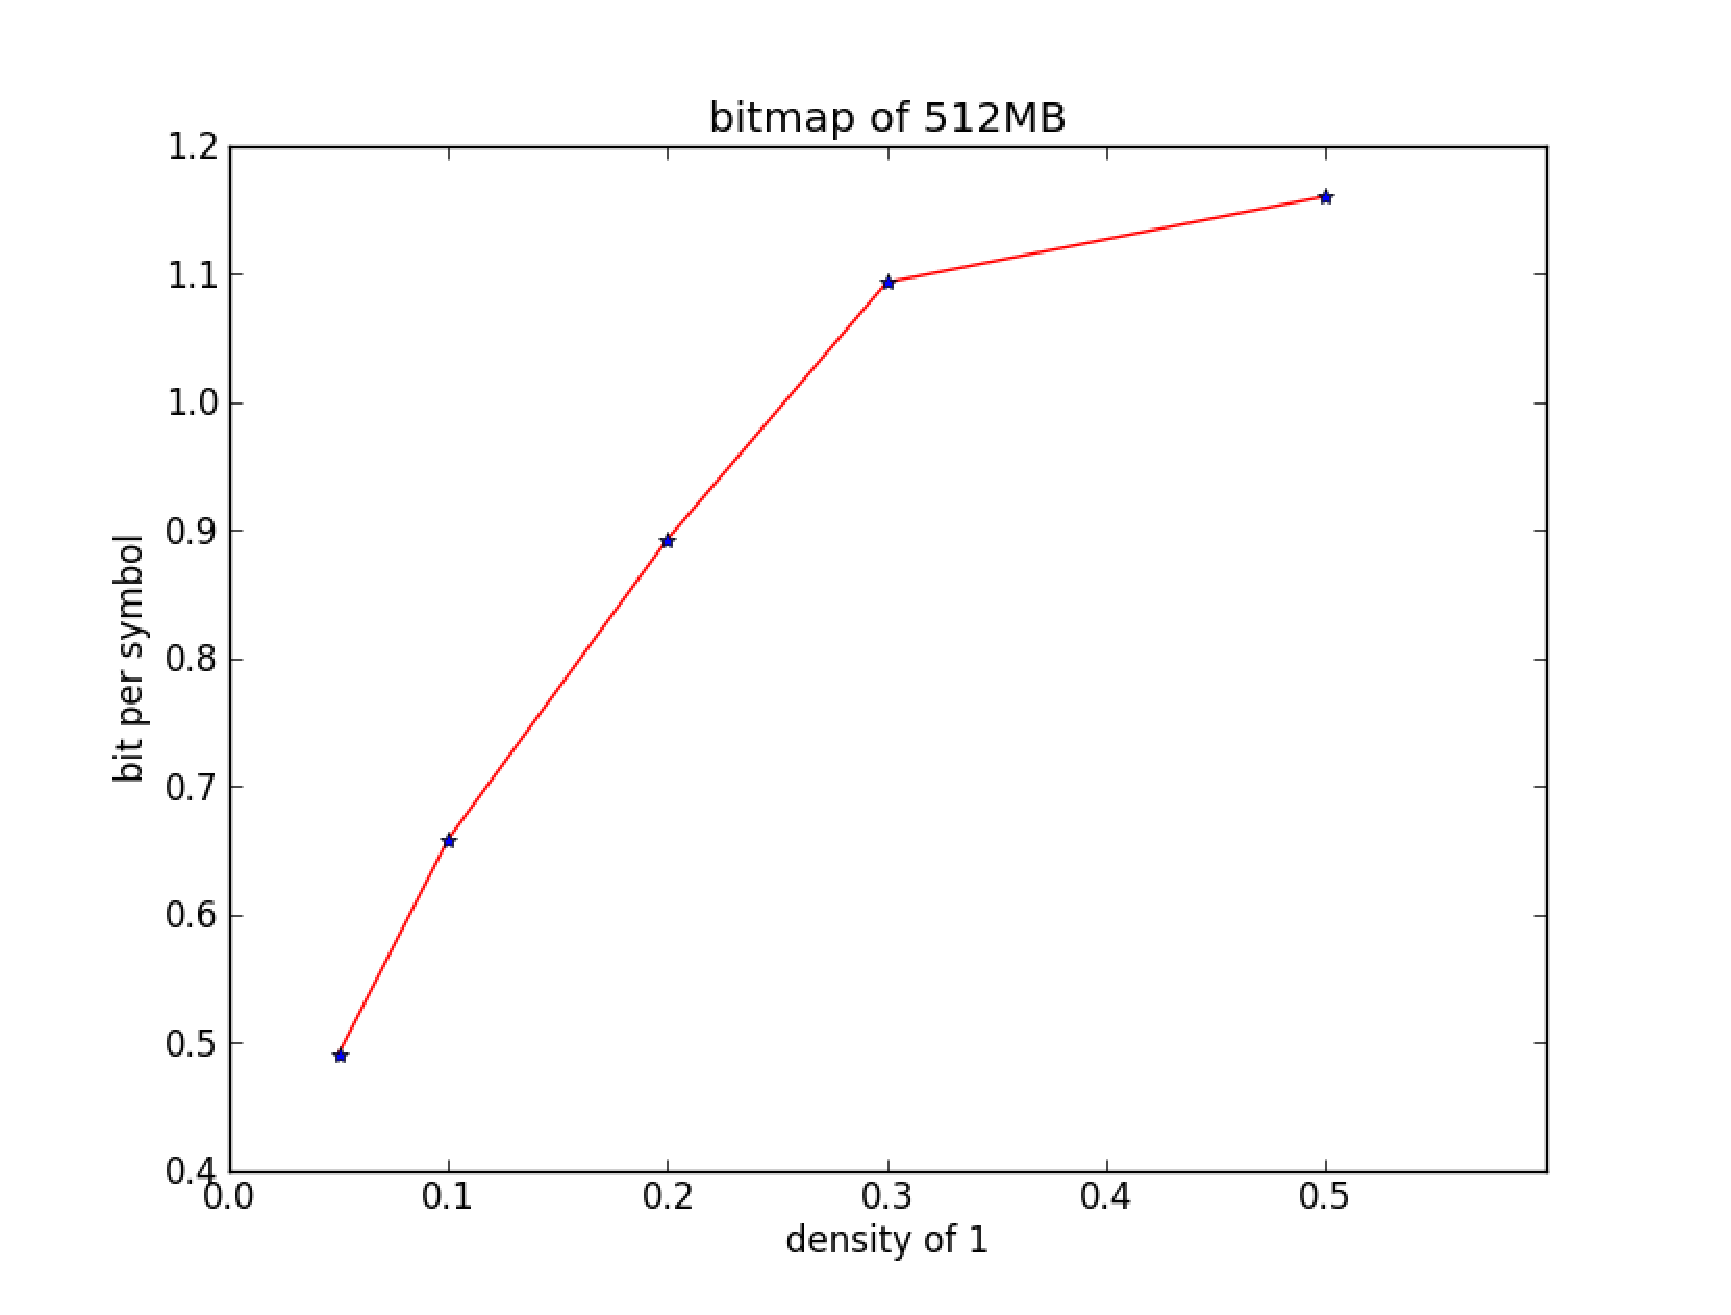
\includegraphics[width=0.8\textwidth]{rrr}
    \caption{RRR方法压缩率随序列经验熵的变化曲线}
\end{figure}


除了经典的RRR方法之外,近年来还出现了一些很有效的rank\&select数据结构实现\cite{okanohara2007practical},其中esp,recrank,vcode以及
sdarray都是类似于RRR方法,bit per symbol有可能达到小于1的实现。这些方法的性能表现在文献\cite{claude2009practical}和文
献\cite{okanohara2007practical}中都有详尽的叙述,这里只展示在空间占用上RRR方法和这几种方法的对比。

\begin{table}[htbp]
    \caption{RRR方法和其他几种方法的压缩效率对比}
    \label{tab:tabcom}
    \centering
    \begin{tabular}{lr}
    \toprule
    数据结构&Bit Per Symbol\\
    \midrule
    rrr&0.48\\
    sdarray&2.05\\
    recrank&1.25\\
    esp&0.50\\
    \bottomrule
    \end{tabular}
\end{table}

表\ref{tab:tabcom}中列出了几种方法和RRR方法的bit per symbol的大小对比,数据来源是论文\cite{claude2009practical},其测试数据是
500M的01序列,1的比例是5\%。在这一条件下,可以看到RRR方法具有明显的空间优势,其压缩率是最高的。

通过对RRR方法实现并和Jacobson的方法做实验对比,可知,在01序列并不均匀时,采用RRR方法具有明显的空间优势。而压缩后缀数组的
实现中所用得到的支持rank操作的字典则都是01序列不均匀分布的,所以在CSA中采用RRR方法实现rank操作会有更好的空间效果。Select操
作的实现是在rank的基础上实现的,总的时间复杂度可以看作rank操作的整数倍。在select操作相对于rank操作较少时,具有较好的表现。
RRR方式总体的效果是比较理想的,尤其是在空间占用上具有很大的优势,在实际应用中,若01序列的分布是很悬殊的,则RRR将是很可取的
一种rank\&select操作实现。

\section{压缩后缀数组和模式匹配}
\subsection{CSA前向搜索模式匹配算法}
从上一节对CSA性质的介绍中,我们知道后缀$T_{SA[\alpha(c)]},T_{SA[\alpha(c)+1]}\ldots T_{SA[\alpha(c)+\beta(c)-1]}$的首字符都
是$c$。设需要搜索的模式为$P[0\ldots m-1]$,首先对于字符$P[0]$,明显的其对应的在$T$中出现的位置为
$SA[\alpha(c)],SA[\alpha(c)+1]\ldots SA[\alpha(c)+\beta(c)-1]$,这个位置集可以表示为$SA[\alpha(c)\ldots\alpha(c)+\beta(c)-1]$,计为
$(l,r)$,称为后缀范围(suffix range)。下一步搜索$P[1]$,即检测$T[SA[\alpha(P[0])]+1],T[SA[\alpha(P[0])+1]+1],\cdots ,T[SA[\alpha(P[0])+\beta(P[0])-1]+1]$
是否等于$P[1]$。由后缀数组的性质可知,这一步的结果得到的后缀数组的下标依然是连续的。以此类推,直到模式串中最后一个字
符搜索完毕,即可得到匹配结果。

近一步观察上面的比较,可以发现,比较$T[SA[\alpha(P[0])]+1],T[SA[\alpha(P[0])+1]+1],\cdots ,T[SA[\alpha(P[0])+\beta(P[0])-1]+1]$
是否等于$P[1]$时并不需要比较字符串。因为$P[1]$对应的也有一个序列$SA[\alpha(P[1])],SA[\alpha(P[1])+1],\cdots ,SA[\alpha(P[1])+\beta(P[1])-1]$,所以只需要求出
$SA[\alpha(P[0])]+1,SA[\alpha(P[0])+1]+1,\cdots ,SA[\alpha(P[0])+\beta(P[0])-1]+1$和$SA[\alpha(P[1])],SA[\alpha(P[1])+1],\cdots ,SA[\alpha(P[1])+\beta(P[1])-1]$
的交集即为模式串$P[1]P[2]$出现的位置。

在上面的迭代过程中要求$SA[\alpha(P[0])]+1,SA[\alpha(P[0])+1]+1,\cdots ,SA[\alpha(P[0])+\beta(P[0])-1]+1$和$SA[\alpha(P[1])],SA[\alpha(P[1])+1],\cdots ,SA[\alpha(P[1])+\beta(P[1])-1]$的交集。
实际计算中无需求出相应的$SA$值,只需求出其对应后缀范围的交集即可,此时可以利用压缩后缀数组的性质$SA[i]+1=SA[\Phi[i]]$,
所以在计算中只需计算$\alpha(P[1]),\alpha(P[1])+1,\cdots , \alpha(P[1])+\beta(P[1])-1$和$\Phi[\alpha(P[0])],\Phi[\alpha(P[0])+1],\cdots , \Phi[\alpha(P[0])+\beta(P[0])-1]$
的交集即可。以此类推,可得到模式串$P$的后缀数组范围。

具体的算法描述如算法\ref{alg:forwardsearch}。

\begin{algorithm}
    \caption{前向搜索模式匹配}
    \label{alg:forwardsearch}
    \begin{algorithmic}[1]
        \Require $P,\Phi,\alpha,\beta$
        \Ensure $(l,r)$
        \Function{forwardSearch}{$P,\Phi,\alpha,\beta$}
        \State $m \gets size(P)$
        \State $n \gets size(CSA)$
        \State $(l,r) \gets (\alpha(P[0]),\alpha(P[0])+\beta(P[0])-1)$
        \For {$i \gets 1$ to $m-1$}
            \State $(l_{tmp},r_{tmp}) \gets (\alpha(P[i]),\alpha(P[i])+\beta(P[i])-1)$
            \For {$j \gets l$ to $r$}
            \If{$\Phi[j] \in (l_{tmp},r_{tmp})$}
                \State $l\gets j$
                \State break
            \EndIf
            \EndFor
            \For {$j \gets r$ down to $l$}
            \If{$\Phi[j] \in (l_{tmp},r_{tmp})$}
                \State $r\gets j$
                \State break
            \EndIf
            \EndFor
            \If{$l > r$}
                \State \Return $\varnothing$
            \EndIf
        \EndFor
        \State \Return $(l,r)$
        \EndFunction
    \end{algorithmic}
\end{algorithm}

算法\ref{alg:forwardsearch}的搜索过程和基于后缀数组的模式匹配算法是等价的。只是这里利用了$\Phi$数组的特性,总的时间复杂度
依然是$O(m\log n)$。

\subsection{CSA后向搜索模式匹配}
压缩后缀数组上的后向搜索模式匹配算法是由Sadakan最早提出来的\cite{sadakane2002succinct}。如上文中所述,我们用$(l,r)$
表示一个模式串在$T$上的后缀位置,模式匹配的目的正是要找到$P$的$(l,r)$。首先,计算$P[m]$的后缀位置,很明显$(\alpha(P[m]),
\alpha(P[m])+\beta(P[m])-1)$就是。假设一般情况,我们已经知道$P[i+1\ldots m-1]$的后缀数组位置为$(l_{P_{i+1}},r_{P_{i+1}})$,
那么$P[i\ldots,m-1]$的后缀数组位置$(l_{P_i},r_{P_i})$必定是由$P[i]$的后缀数组位置的一部分组成的,设$P[i]$的后缀数组位置
为$(l_{P[i]},r_{P_i})$,那么对于$l_{P[i]\leq k \leq r_{P_i}}$只要$SA^{-1}SA[k]+1$在$(l_{P_{i+1}},r_{P_{i+1}})$中,$k$一定在$(l_{P_i},r_{P_i})$
中。也就是说$P[i\ldots n-1]$的出现位置一定是$P[i]$的出现位置后面紧跟着$P[i+1\ldots m-1]$的出现位置。加上$\Phi[i]=SA^{-1}[SA[i]+1]$,
所以我们可以得到公式\ref{equa:equa1}。

\begin{equation}\label{equa:equa1}
    k \in (l_{P_i},r_{P_i}) \iff k \in (l_{P[i]},r_{P[i]}) \wedge \Phi[k] \in (l_{P_{i+1}},r_{P_{i+1}})
\end{equation}

由于在简明数据结构存储下$\Phi$可以在常数时间内获得,并且其值在$(l_{P_{i+1}},r_{P_{i+1}})$上是递增的,所以,可以用二分搜索
来搜索$\Phi[k]$是否在$(l_{P_{i+1}},r_{P_{i+1}})$上,时间复杂度是$O(\log n)$。重复上述过程$m$次,即可在CSA上用$O(m\log n)$
时间复杂度找到模式$P[0\ldots m-1]$的后缀数组范围$(l,r)$

算法\ref{alg:backwardsearch}给出了CSA上的后向搜索的伪代码。而图\ref{figbackwardsearch}给出了一个采用算法\ref{alg:backwardsearch}
的例子,搜索模式$P=CCAGTA$。每一个方块儿对应一个字符的后缀数组区域,灰色的区域表示对应$P$的一个后缀在$T$的后缀数组上的位置
范围。在右起第二步,计算新的区域时,根据下一个字符$G$的后缀范围,计算其$\Phi$值,查看这个$\Phi$是否落在当前模式$TA$的后缀范
围内,由于$\Phi$的递增特性,很容易用二分搜索方法找到新的区域的上下界。

\begin{algorithm}
    \caption{后向搜索}
    \label{alg:backwardsearch}
    \begin{algorithmic}[1]
        \Require $P,\Phi,\alpha,\beta$
        \Ensure $(l,r)$
        \Function{backwardSearch}{$P,\Phi,\alpha,\beta$}
        \State $l_{m} \gets 0;r_{m}\gets n-1$
        \For {$i\gets m-1$ down to $0$}
            \State $l_i \gets \min\{ k \in [\alpha(P[i]),\alpha(P[i])+\beta(P[i])-1],\Phi[k] \in [l_{i+1},r_{i+1}]\}$
            \State $r_i \gets \max\{ k \in [\alpha(P[i]),\alpha(P[i])+\beta(P[i])-1],\Phi[k] \in [l_{i+1},r_{i+1}]\}$
            \If{$l> r$}
                \State \Return $\varnothing$
            \EndIf
        \EndFor
        \State \Return $(l_0,r_0)$
        \EndFunction
    \end{algorithmic}
\end{algorithm}


\begin{figure}[t]
    \centering
    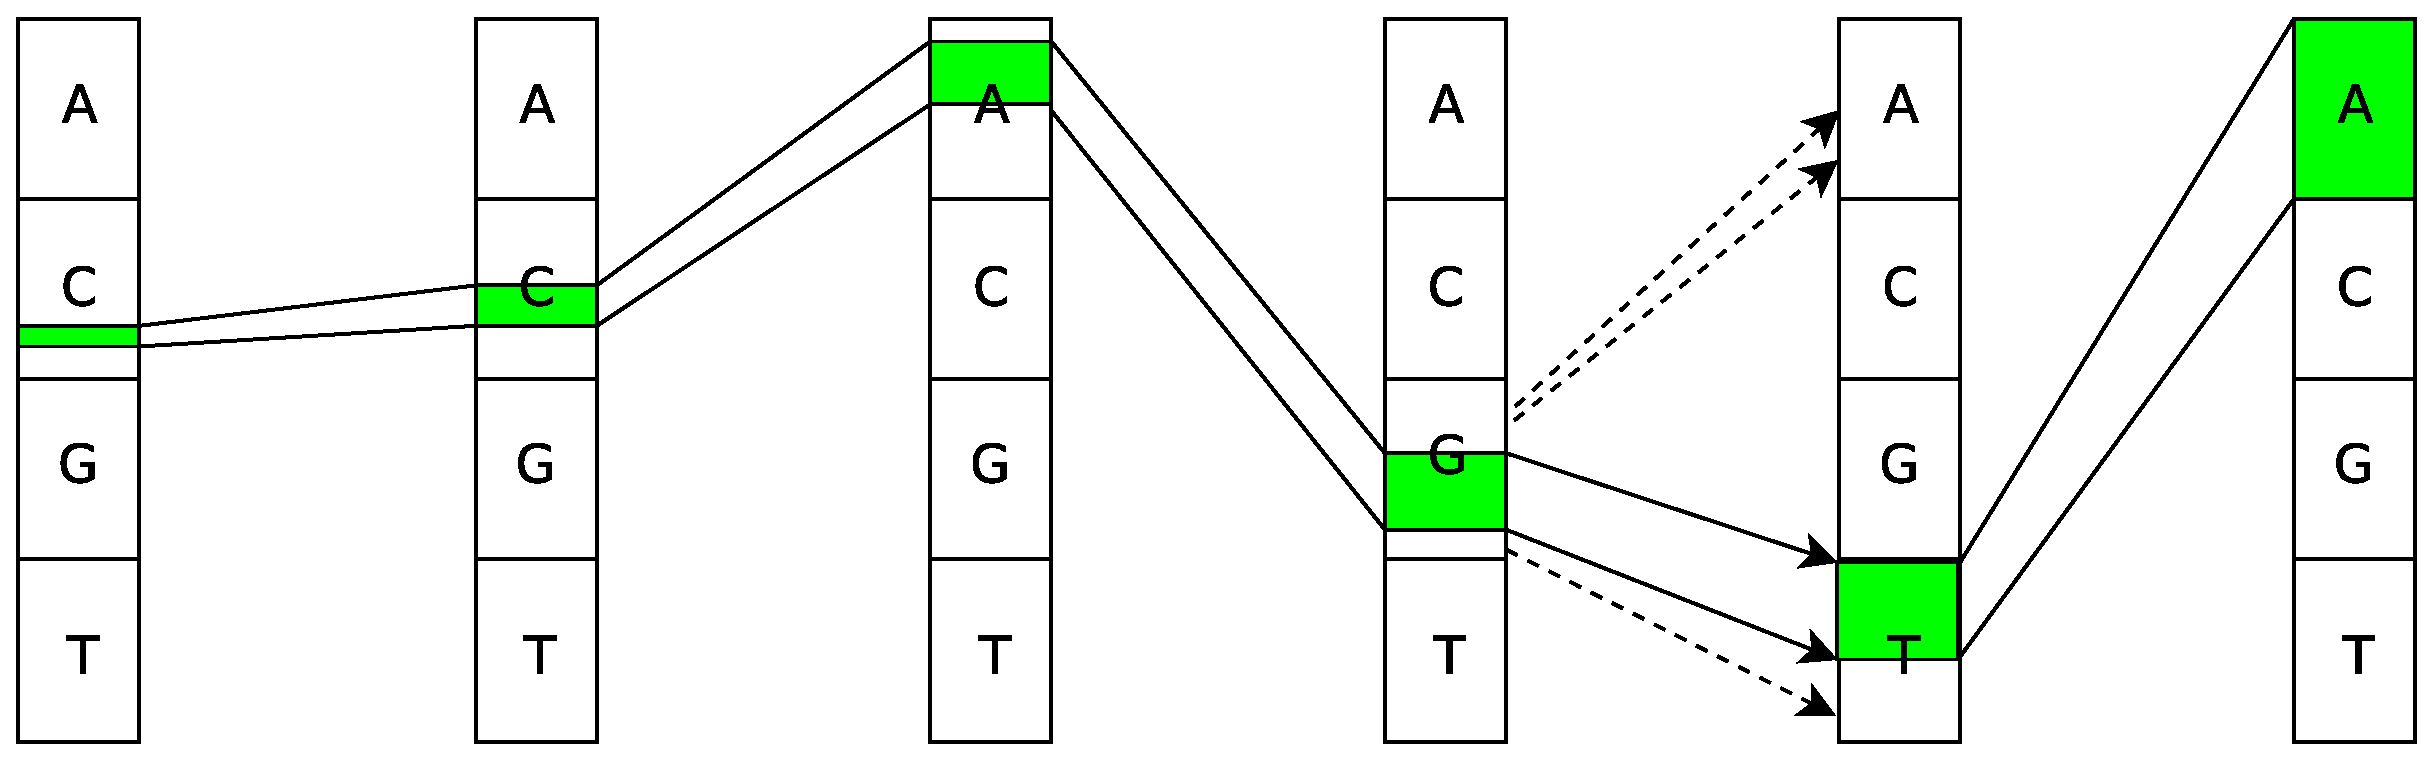
\includegraphics[width=0.7\textwidth]{csa_backwardsearch}
    \caption{CSA上的后向搜索}
    \label{figbackwardsearch}
\end{figure}

\section{压缩后缀数组和自索引}
压缩后缀数组优于后缀数组的另一性质是其自索引性。在上一小节的模式匹配算法中,可以看到并不需要原文本$T$即可完成匹配,
基于这个原理,只要给压缩后缀数组添加一个辅助数组即可实现压缩后缀数组的自索引算法。

考虑已知$\Sigma$中任意字符$c$的$\alpha(c)$值,则$\beta(c)=\alpha(c+1)-\alpha(c)$,所以只需保存$\alpha(c)$即可完成
无需原文本的模式匹配,基于此在压缩后缀数组基础上增加一个辅助数组$\alpha$即可实现自索引。

考虑下面的性质$T[SA[\alpha(c)]]=T[SA[\alpha(c)+1]]=\cdots=T[SA[\alpha(c)+\beta(c)-1]]=c$,所以对于$T$中任意位置$i$处
的字符,只要求出其对应后缀$T_i$的名次,即$j=SA^{-1}[i]$,便可在$\alpha$数组中搜索其所在区间使得对某个字符$c$存
在$\alpha(c)\leq j< \alpha(c+1)$,即得到$T[SA[j]]=c$,所以即可知$T[i]=c$。而由前文中可所述$\Phi$的性质可知后缀数组的
逆数组$SA^{-1}$是可以在线性时间内得到的。

按照上面叙述的方法可以很方便的恢复出文本$T$的任意字符,进而恢复出$T$的任意长的子串$T_{i,j}$。在实际运算中
考虑到压缩后缀数组的性质$SA^{-1}[i+1]=\Phi[SA^{-1}[i]]$,所以在已知$SA_[i]$求出$T[i]$的情况下求$T[i+1]$时,
不必再求$SA^{-1}[i+1]$,直接返回$\Phi[SA^{-1}[i]]$,这个计算是常数时间的,而不是线性时间\cite{sadakane2000compressed}。

具体算法如算法\ref{alg:getT}。

\begin{algorithm}
    \caption{CSA自索引}
    \label{alg:getT}
    \begin{algorithmic}[1]
        \Require $\Phi,\alpha,i,j$
        \Ensure $T[i\ldots j]$
        \For {$k\gets i$ to $j$}
            \If {k=i}
                \State $rank \gets SA^{-1}[k]$
                \State $prev \gets rank$
            \Else
                \State $rank \gets \Phi[prev]$
            \EndIf
            \State $T[k] \gets$ \Call{binarySearch}{$rank$,$\alpha$}
        \EndFor
        \State \Return $T[i\ldots j]$
    \end{algorithmic}
\end{algorithm}

上述算法总共执行$m=j-i+1$步,每一步执行一次$|\Sigma|$上的二分搜索,且要求$SA$,所以时间复杂度为
$O(\log |\Sigma|+\log \log n)$,所以总的时间复杂度为$O(m(\log |\Sigma|+\log \log n))$。

\section{本章小结}
本章主要在前面阐述的后缀数组和压缩后缀数组性质的基础上提出了基于压缩后缀数组的文本索引和自索引算法。并详细介绍了上实现压缩
后缀数组的基本数据结构:RRR算法。之后介绍了两种CSA上的$O(m\log n)$时间复杂度的模式匹配算法:前向搜索和后向搜索。为下一章的
DNA序列比对算法给出实现基础。最后还介绍了CSA的自索引性质,并给了由压缩后缀数组恢复原文本序列的算法。

    
\chapter{基于压缩后缀数组的序列比对算法}
CSA短读比对算法(CSAA)采用CSA索引参考序列,利用CSA的后向搜索完成匹配过程。CSA的后向搜索是一种精确匹配算法,由于
DNA序列存在变异,以及测序技术有一定的错误率,所以不能简单的使用精确搜索算法。本文提出了两种策略来实现短读比对中的非精确匹配
要求。一是在后向搜索过程中引入了搜索树,使得在搜索过程中可以随时对短读序列进行插入,删除,替换等操作。另一种策略是
采用类似优先队列的数据结构,这一数据结构结合打分机制保证在后向搜索的每一步中都是沿着最优的搜索方向前进,并且采用分支限界
的策略适时淘汰很差的搜索方向。


\subsection{精确匹配}

精确匹配是后向搜索的具体实现。设$T$为长为$n$的参考序列,$P$为测序得到的短读序列中的一个短读,长为$m$。将$P$
映射到$T$上的方法如算法\ref{alg:exac}所示。

\begin{algorithm}
    \caption{精确匹配}
    \label{alg:exac}
    \begin{algorithmic}[1]
        \Require $T,csa,P$
        \Ensure $(l,r)$
        \Function{ExactMatch}{$csa,P$}
        \State $l \gets csa.\alpha(P[m-1])$
        \State $r \gets csa.\alpha(P[m-1])+\beta(P[m-1])-1$
        \For{$i=m-2 \to 0$}
            \If{$l>r$}
                \State \Return $\phi$
            \EndIf
            \State $(l,r) \gets$ \Call{backwardSearch}{$l,r,P[i],csa.\alpha,csa.\beta$}
        \EndFor
        \State \Return $(l,r)$
        \EndFunction
    \end{algorithmic}
\end{algorithm}

算法\ref{alg:exac}采用后向搜索把短读精确匹配到参考序上,返回短读的后缀数组位置$(l,r)$,再利用CSA可以求得$(l,r)$
对应的$T$上的真正位置,完成映射。由于是精确匹配,就只有两种结果,要么匹配上,要么没匹配上,就无需打分机制。这种匹配
方式是完全匹配,但并不适合大多数存在变异和测序误差的短读序列。本文提出的CSAA算法是建立在非精确匹配的基础上的。

\subsection{近似匹配}

由于同一物种之间存在的个体差异以及测序技术存在的误差,Resequencing技术得到的短读序列和该物种的标准参考序列之间
必然存在着不同,这会造成即使同一种基因序列也无法完全比对映射到参考序列上。所以对短读和参考序列之间的比对
仅仅精确比对映射是远远不够的,这会造成大量的短读因为相差一两个碱基而不能映射到参考序列上,而这一两个碱基很可能
是测序误差或者生物个体之间的SNP造成的,不应当认为二者是不能匹配的。所以,采用合适的非精确比对算法是必须的。本文提出的
非精确匹配算法中,支持对短读进行替换(substitude),插入(insert),删除(delete)三种变换操作,通过这三种变换可以保证
变异的或者发生测序错误的短读序列依然能正确匹配到参考序列的合适位置上。

考虑一个给定的长为$m$的短读序列$P$,采用后向搜索,当搜索到第$i+1$个位置时,得到序列$P_{i+1}$的后缀数组位置$(l_{i+1},r_{i+1})$,
依照精确匹配的算法下一步应当在$(l_{i+1},r_{i+1})$的基础上搜索字符$P[i]$,从而得到一个新的后缀数组位置$(l_i,r_i)$。在此,如果我们不
搜索$P[i]$,而是搜索另一个符号$c \neq P[i]$,得到另一个后缀数组位置$(l_{i}^{'},r_{i}^{'})$。接着在$(l_{i}^{'},r_{i}^{'})$基础
上继续搜索$P[0\ldots i-1]$,那么最终得到后缀数组位置$(l_0,r_0)$将不再是序列$P$的一个后缀数组位置了,而是将$P[i]$替换为$c$
后的新字符串的后缀数组位置。称这个新位置为$P$的一个替换近似串的后缀数组位置,计为$(l_0,r_0,m,P(S_i))$,即长为$m$的序列$P$在
$i$位置进行一次替换后可以映射到参考序列的后缀数组位置$(l_0,r_0)$。

图\ref{fig:substitude}给出了把短读序列中的一个符号$T$替换为$A$时的搜索过程,实线为精确匹配的过程,虚线是替换后的搜索过程。

\begin{figure}[htb]
    \centering
    \includegraphics[width=9cm]{substitude.eps}
    \caption{替换操作示例} \label{fig:substitude}
\end{figure}

不同于替换操作,如果在搜索到$P[i]$时,放弃搜索$P[i]$符号,直接在$(l_{i+1},r_{i+1})$的基础上搜索序列$P[0\ldots i-1]$,那么
最终得到的后缀数组位置$(l_0,r_0)$将是$P$删除$P[i]$后的近似串在参考序列上的后缀数组位置,计为$(l_0,r_0,m,P(D_i))$,,即长为$m$
的序列$P$在$i$位置进行一次删除后可以映射到参考序列的后缀数组位置$(l_0,r_0)$。

如图\ref{fig:delete}所示为删除短读序列中的一个符号后的搜索过程。

\begin{figure}[htb]
    \centering
    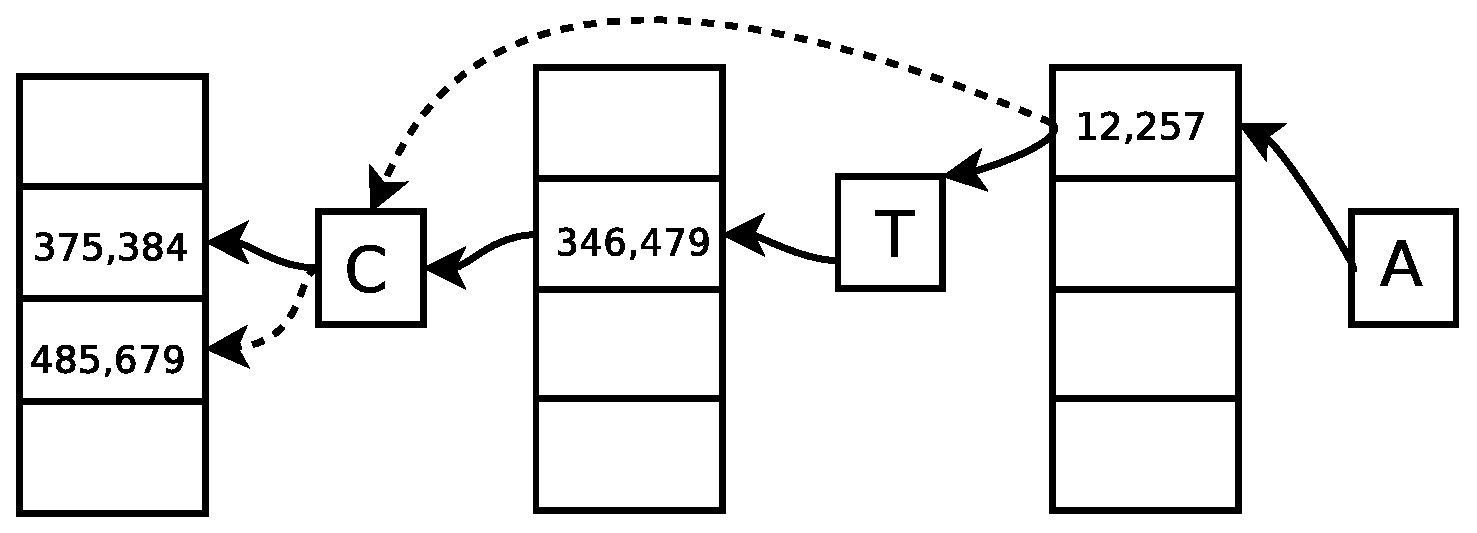
\includegraphics[width=9cm]{delete.eps}
    \caption{删除操作示例} \label{fig:delete}
\end{figure}

对于插入操作,在搜索到$P[i]$时,不直接搜索$P[i]$,而是在$l_{i-1},r_{i-1}$的基础上搜索符号$c$,得到$(l_{i}^{'},r_{i}^{'})$,接着
在此基础上搜索序列$P[0\ldots i]$,最终得到的后缀数组位置$(l_0,r_0)$将是$P$在$i$位置插入符号$c$后的近似序列的后缀数组位置。计为
$(l_0,r_0,m,P(Ii)$,即长为$m$的序列$P$在$i$位置插入一个符号后可以映射到参考序列的后缀数组位置$(l_0,r_0)$。

如图\ref{fig:insert}所示为插入一个符号'A'前后的短读序列中的一个符号后的搜索过程。

\begin{figure}[htb]
    \centering
    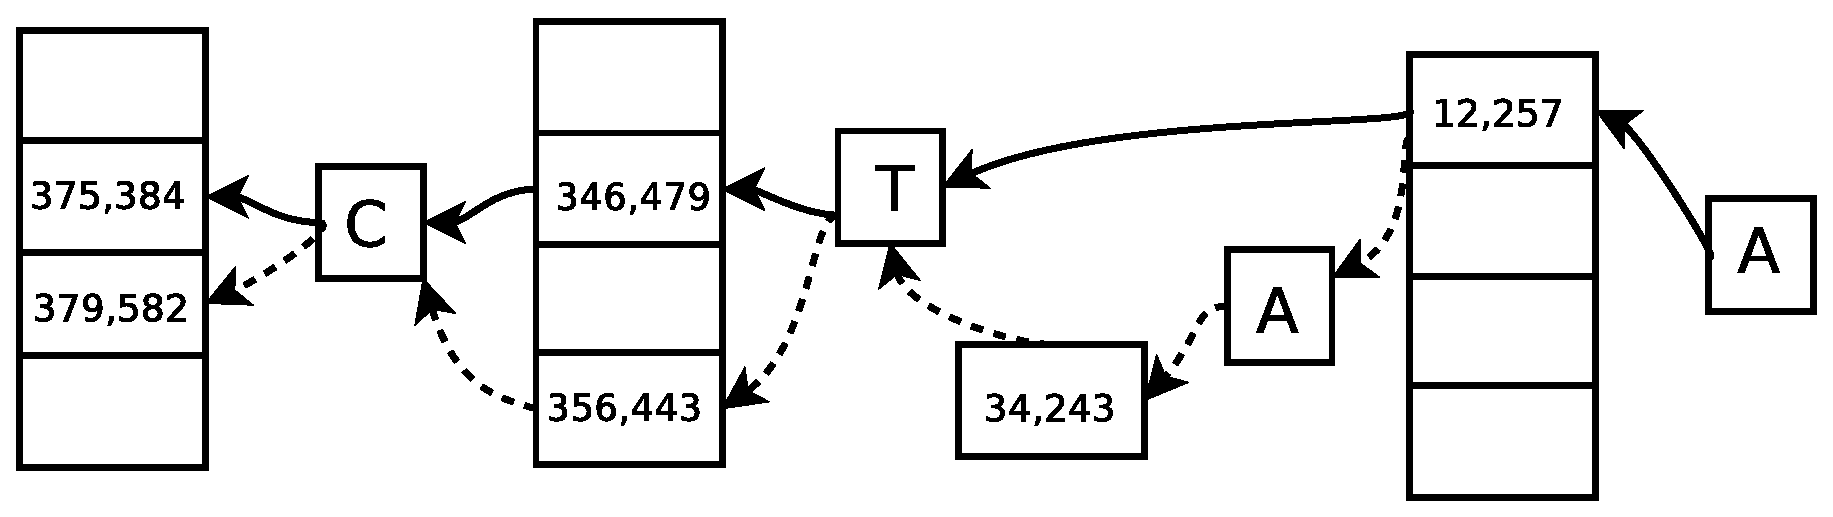
\includegraphics[width=9cm]{insert.eps}
    \caption{插入操作示例} \label{fig:insert}
\end{figure}

\subsubsection{搜索树}

按照上文中描述的用后向搜索实现替换,删除,插入操作的方法,要实现短读序列的近似匹配,在不知道具体的替换,删除以及插入
位置时,需要在每一次后向搜索一个符号时都分别做一次替换,删除,插入操作。而每一次操作实际上都导致了一个新的近似序列的产生,在
未完成整个序列的搜索时,最终哪一个近似序列能够较好的映射到参考序列上依然是未知的,这就要求我们在搜索过程中保留每一个可能的近
似序列。

\begin{figure}[htb]
    \centering
    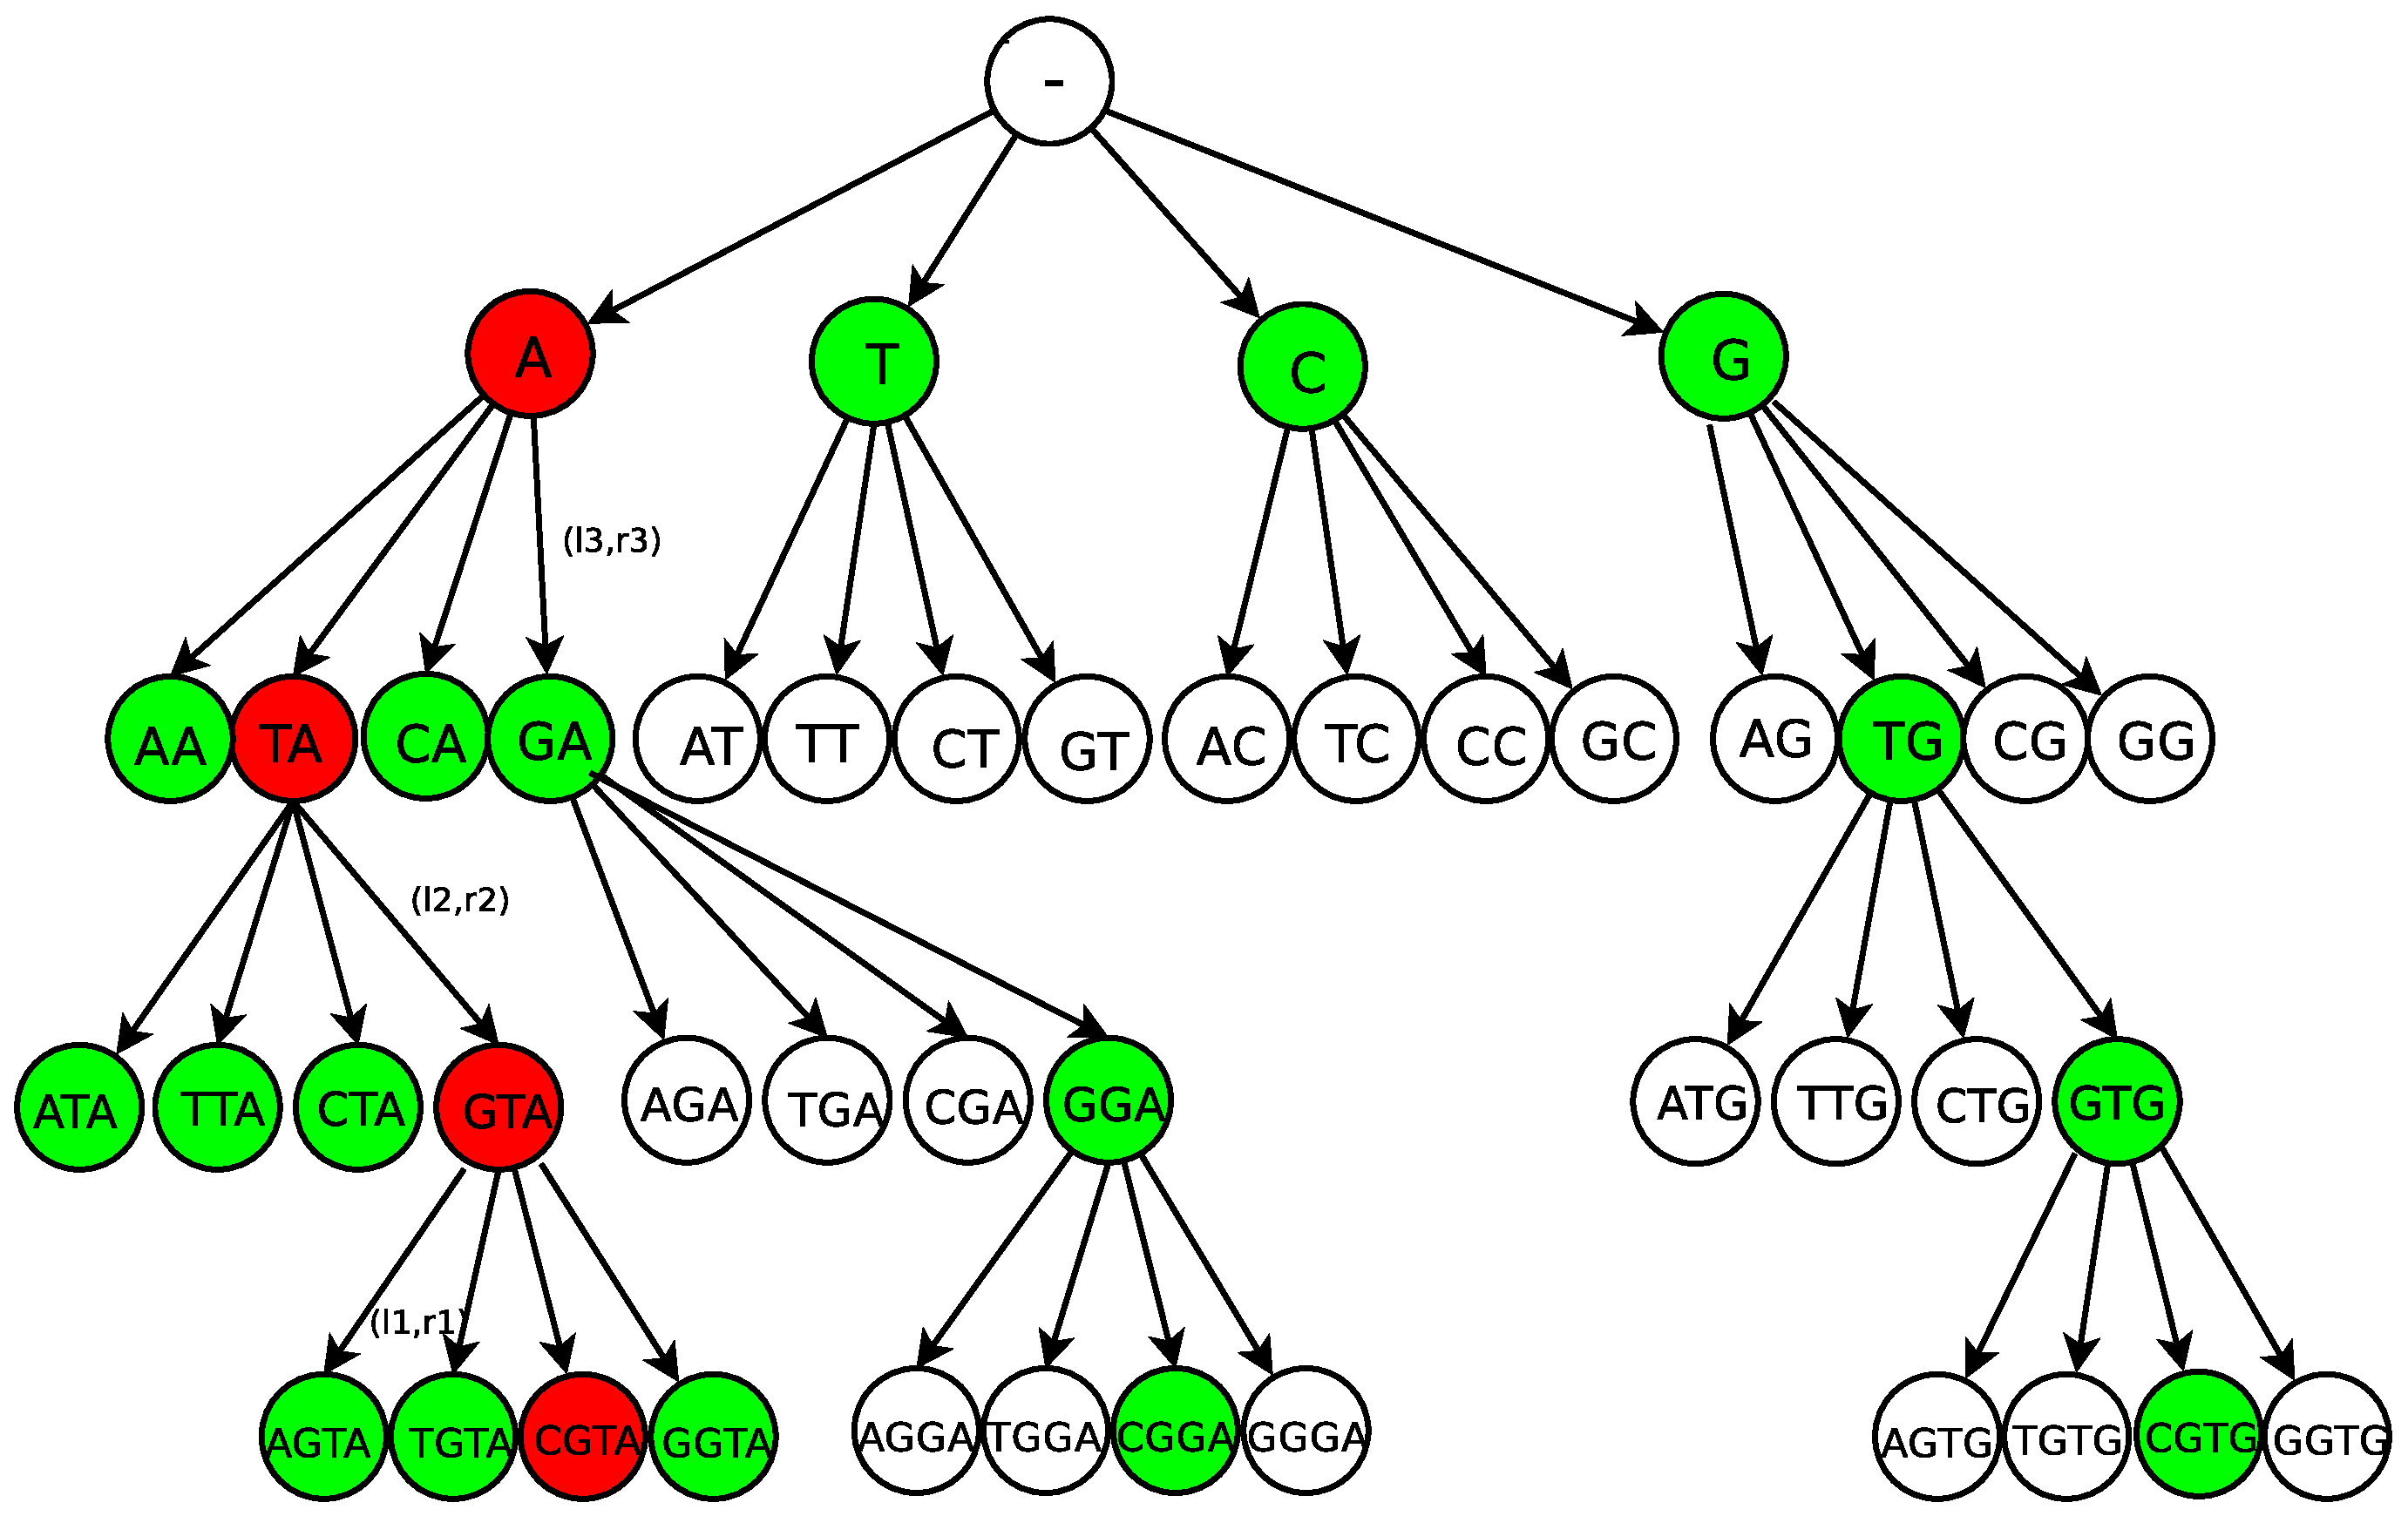
\includegraphics[width=12cm]{searchtree.eps}
    \caption{近似匹配示例} \label{fig:searchtree}
\end{figure}

实际上,每一次的替换,删除或者插入操作导致的新的近似序列可以看作一个树上的遍历过程。如图\ref{fig:searchtree}所示,对于一个长
为4的短读 $P=$``CGTA''的搜索过程,简化起见,省略了删除和插入操作。首先通过CSA查询$P[3]=$`A'在参考序列上的后缀数组位置。接着把
$P[3]=$`A'分别替换为`T',`C',`G',在CSA上查找替换后的后缀数组位置。图中红色路径标志的是到当前搜索深度没有替换操作的近似串,而
绿色标记的则是到当前深度有一次替换操作的近似串,无色的是有两次以上替换操作的近似串搜索路径。可以看到,随着搜索深度的增加,搜索
的方向急剧扩大,加上还有未画出的删除和插入操作,可能的搜索方向会更多。

搜索树的本质是对每一个可能的近似序列都进行搜索,假设一个短读序列的长度为$m$,因为每一个位置都有4种替换,4种插入和1种删除
方法,则总共有$9^m$个近似串。考虑到$m$一般在20到70之间,
如果直接采用搜索树来进行近似匹配,搜索规模会非常大而难以在有效时间内实现。实际上也无需比对所有的近似串,对于某些替换,删除或者插入操作过多的近似串,
应该提前抛弃掉,即采用分支限界法来对搜索树进行剪枝。

\subsubsection{分支限界}

搜索树的规模是指数级增长的,因此必须进行适当的剪枝,抛弃一些没有价值的搜索方向。传统的DNA序列比对中用到了编辑距离,汉明距离
等来度量两个序列的相似度。在此我们也可以使用类似的方法做分支限界,比如采用编辑距离做分支限界。给定一个最大编辑距离$maxdistance$,
当在短读序列$P$上后向搜索进行到第$i$步时,在某个搜索方向上的一个近似序列为$P^{'}$,计算$P$和$P^{'}$之间的编辑距离,若距离大于预先
定义的$maxdistance$,则抛弃这个搜索方向,否则,继续。汉明距离做分支限界的方法和编辑距离方法类似。

采用编辑距离和汉明距离的方法必须对每一个得到的近似序列和短读序列计算距离,这会导致算法效率的降低。实际上,可以采用罚分机制取
代每次都计算编辑距离的开销。在搜索树上向前搜索时,每一次替换,删除或者插入操作都会产生一个新的近似序列,这个序列做了多少次变
换操作是已知的,预定义每一个indel操作的罚分,每一次操作都会对这个近似序列增加相应的罚分,当罚分达到一个预定义的最大罚分
$maxpenalty$
时,即认为这个近似序列已经和短读序列相似度太小,没有必要再搜索下去了。通过这样的罚分机制,可以去除较差的近似序列,而无需
每次都计算编辑距离。

在生物信息学领域,一个indel称为一个空位,对应的罚分称为空位罚分。通常连续的空位的罚分不能简单的做线性增加来处理。
Affine gap penalties是生物信息学领域常用的一种罚分机制,假设有一个连续gap长为$x$,则这个gap的罚分为$-(\rho +\sigma x)$,其中
$\rho >0$,$\sigma$是每一个indel操作的罚分。

除了罚分机制,在论文\cite{li2009fast}中,作者还提出了一种新的高效的分支限界策略,称之为$D(.)$数组。在论文作者实现的短读比对
软件$BWA$中也使用了这一策略来限制搜索空间增长。$D(.)$数组是一个和序列串$P$等长的一个整数数组,$D[i]$取决于序列串$P$的后缀
$P_i$是否是参考序列$T$的一个子串,是的话则增加,不是则归0。具体过程如算法\ref{alg:darray}所示。

\begin{algorithm}
    \caption{计算$D(.)$数组}
    \label{alg:darray}
    \begin{algorithmic}[1]
        \Require $T,csa,P$
        \Ensure $D(.)$
        \Function{CalculateD}{$csa,P$}
            \State $z \gets 0$
            \State $j \gets 0$
            \For{$i \gets 0$ to $|P|-1$}
                \If{$P[j\ldots i]$ is not a substring of $T$}
                    \State $z \gets z+1$
                    \State $j \gets i+1$
                \EndIf
                \State $D[i] \gets z$
            \EndFor
        \EndFunction
    \end{algorithmic}
\end{algorithm}

$D(.)$数组的作用,是结合每一个近似序列的一个辅助值$z$来分支限界的。开始搜索时,序列$P$的$z$值是$D[m-1]$,由算法\ref{alg:darray}
可知,此时的$z$值是$D(.)$数组中最大的值,并且反映了整个序列$P$有多少个连续子串是参考序列的子串。其后在搜索中每进行一次替换,
删除或者插入操作,$z$值都会减小。当搜索到第$i$个位置导致$z<D[i]$时,这个搜索方向将被抛弃。采用$D(.)$数组能够进一步的缩小搜索
空间,提高效率。本文实现的CSAA软件中也把$D(.)$数组作为一个重要的分支限界条件来使用,并取得了较好的结果。

综上所述,本文提出的结合$D(.)$数组和罚分机制做分支限界的搜索树近似匹配算法如下:

\begin{algorithm}[H]
    \caption{近似匹配}
    \label{alg:appro}
    \begin{algorithmic}[1]
        \Require $T,csa,P,maxpenalty$
        \Ensure $\{(l,r)\}$
        \Function{ApproMatch}{$P,i,l,r,z,penalty$}
            \If{$z<D[i]$}
                \State \Return $\phi$
            \EndIf
            \If{$penalty>maxpenalty$}
                \State \Return $\phi$
            \EndIf
            \If{$i<0$}
                \State \Return (l,r)
            \EndIf
            \State $S \gets \phi$
            \State $S \gets S\ \cup$\ \Call{ApproMatch}{$P,i-1,l,r,z-1,penalty+delPenalty$}
            \ForAll{$b \in \{A,T,C,G\}$}
                \State $(l,r)\gets$\Call{backwardSearch}{$l,r,b,csa.\alpha,csa.\beta$}
                \If{$l\leq r$}
                \State $S \gets S\ \cup\ $ \Call{ApproMatch}{$P,i,l,r,z-1,penalty+insPenalty$}
                    \If {$b=P[i]$}
                    \State $S \gets S\ \cup$\ \Call{ApproMatch}{$P,i-1,l,r,z,penalty$}
                    \Else
                    \State $S \gets S\ \cup$\ \Call{ApproMatch}{$P,i-1,l,r,z-1,penalty+subPenalty$}
                    \EndIf
                \EndIf
            \EndFor
            \State \Return $S$
        \EndFunction
    \end{algorithmic}
\end{algorithm}

算法\ref{alg:appro}是本文提出的CSAA算法的核心,采用两种分支限界策略,减小搜索空间,能够完成替换,插入和删除三种变换操作,
实现近似搜索。算法\ref{alg:appro}同时使用了后向搜索算法\ref{alg:backwardsearch}。该算法只是一个理论形式,具体实现中必须做一些修改。



    \chapter{CSAA的实现}

上文中给出了CSAA的算法过程,实际实现中CSAA采用了一些优化措施,进一步提高程序的效率。这些措施主要是从提高执行效率和准确度
两个方面来考虑的。CSAA主要包括三个子程序:build index,alignment,output。build index子程序完成对参考序列$T$建立压缩后缀数组
索引,对同一个参考序列只需建立一次索引即可。alignment子程序是CSAA的核心,完成对短读序列到参考序列$T$的映射,输出CSAA
自定义的一种SAI格式文件。最终SAI格式文件通过output子程序转为标准比对结果文件SAM(Sequence Alignment/Map format)。

\subsection{效率优化}
在实际应用中,每一个短读一般有20到70个bp,若直接采用递归算法实现,递归深度过深会严重影响程序的执行效率。所以在
CSAA中使用了一种改进的优先队列数据结构来替代递归,把递归转为迭代形式。

优先队列的每一项保存一个近似匹配的序列,按照每个近似序列的质量得分排列。质量得分是对每一个近似序列的评分。初始评
分是对应短读序列不做任何变换时的评分,定义为一个常数,由程序预先定义的最大失配数量,最大gap open数目,最大gap extension
数目决定。这里参照序列比对领域的一些标准定义,对序列做一个替换称为一次失配,一次单独的插入或者删除称为一个gap open。若在
已经gapopen的位置连续执行了一次删除或者插入操作,称为增加了一个gap extension。在CSAA中可以定义程序执行时的最大可允许的失配
,gap open和gap extension数量,以保证近似序列和短读序列之间的近似程度在合理范围之内。CSAA同样的对理论上的罚分机制也做了一些修正,
罚分不再针对替换,插入和删除操作,而是针对近似序列的失配,gap open,gap extension数量罚分。三种操作具有不同的罚分标准。可以
在执行程序时输入,也可以使用默认的罚分标准。每一个短读序列的质量得分也由罚分后的得分决定。

优先队列使用了最大堆来实现,这可以保证较高的效率,另一方面,也可以通过限制优先队列的容量来保证搜索空间在短序列时不会太大。通过
优先队列,可以把算法\ref{alg:appro}描述的深度优先的搜索方向变为广度优先,加上优先队列的大小限制,可以较好的节省内存空间。保证
在较低内存下依然可以运行。

CSAA在实现时考虑到CSA查询后缀数组位置的速度较快,而由后缀数组位置查询实际的映射位置比较慢,同时因为在做近似匹配的过程也无需
具体的映射位置,所以CSAA定义了一个SAI文件,该文件是CSAA的中间输出文件,所存内容为短读序列的近似匹配结果,包括每一个
短读 序列的近似匹配后的后缀数组位置,质量得分,变换操作位置,类型等信息。最终通过CSAA的一个子程序结合参考序列$T$完成SAI
文件到标准的比对文件SAM文件的输出。

\subsection{使用seed提高精确度}
在DNA测序技术中,单端测序和双端测序都存在测序质量的问题。离结合位点越近的位置,测序结果准确率越高,而越远的位置,测序准确率
越低。根据这一现象,关于Bowtie实现的论文\cite{langmead2009ultrafast}中提出了seed的概念,针对短读序列中准确率较高的部分采用较
高的限制。在算法\ref{alg:appro}中,定义当$z>0$时才停止搜索,在CSAA中实际上是分为两部分的,seed部分当$z>minDifference$时就会
抛弃这个搜索方向。而在非seed部分,默认情况下$minDifferecnce=0$。同样的在在seed部分,失配,gap open和gap extension的数量
限制也相较非seed部分较大。通过这样的策略,可以有效提高搜索的精度。至于seed的具体长度,可以根据不同的测序技术来给定。默认情况
下,Bowtie的seed长度是28,随本文发布的CSAA中seed的默认长度是32。

因为seed的限制条件较高,所以如果能首先对seed进行匹配,可以尽早抛弃掉一些不满足seed部分匹配要求但满足非seed部分匹配要求的序列。
但因为seed是在短读序列的前缀部分,而我们使用CSA索引的后向搜索时是从后往前搜索的,最后才搜索seed部分。所以在CSAA中无论是建立
索引还是,还是短读匹配都是对短读的reverse序列进行匹配的。这同BWA的做法一致。

\section{实验测试}

为测试CSAA的性能,本文同时测试了MAQ\cite{li2008mapping},Bowtie\cite{langmead2009ultrafast}和BWA\cite{li2009fast}这三个比对工
具,和CSAA进行比较。分别对比这几个工具在不通规模数据上建立索引时的时间,需要的内存;以及在模拟数据上和真实数据上的比对能力。
MAQ为所有的短读序列建立hash表,进而遍历整个参考序列来实现比对。Bowtie和BWA是用基于BWT的索引建立
的比对工具,其中Bowtie采用了回溯法实现替换操作,但不支持inset和delete操作,即上文中所论述的gap alignment。BWA采用了本文类似的
算法,但在建立索引时,采用了分段建立索引的方法,建立索引的速度比较慢,且需要保存参考序列$T$。

\subsection{测试环境和数据}
在对CSAA的测试中,使用gcc 4.6.3编译链接,并且使用了-O3优化。系统环境为ubuntu 12.04 amd64,运行在一台具有18G内存的工作站上。
测试使用的数据是标准的人类基因组序列hg18.fa,来自1000 Genome Project的NCBI build 36,模拟数据也是在该数据上生成。所有测试数
据均使用默认选项运行。

\subsection{索引建立时间}
表\ref{tab:tab1}中对比了bowtie,BWA和CSAA三种工具分别建立索引时所需要的时间和内存消耗对比情况,表中数据分别对应几个工具在索引
512M,1024M和2048M的数据时所需要的时间和内存。

\begin{table}[htbp]
    \caption{建立索引的时间空间对比}
    \label{tab:tab1}
    \centering
    \begin{tabular}{lrrrrrr}
        \hline
        \multirow{2}{*}{Program} & \multicolumn{3}{c}{Time(s)} & \multicolumn{3}{c}{Memory(M)}\\
        \cline{2-4}
        \cline{5-7}
        & 512M &1024M &2048M &512M &1024M &2048M\\
        \hline
        Bowtie&1311 &2720 &5581 &987 &1109 &1210 \\
        BWA&531 &1101 &2445 &1890 &1902 &2006 \\
        CSAA&413 &843 &2065 &2483 &5325 &11435 \\
        \hline
    \end{tabular}
\end{table}

从表\ref{tab:tab1}中的测试结果可以看到,CSAA相对其他两个不对工具在索引时间上具有较大优势,这是由于BWA和Bowtie都同时给inverted
reference建立了索引,用时会较长。其中Bowtie建立索引时是分块建立索引的,最终再合并成一个索引,时间效率最差,但需用内存空间最小。

\subsection{模拟数据测试}
本文使用SAMtools工具包中的wgsim工具从人类基因组序列中随机生成模拟的短读序列。然后,分别用四种比对工具对这些模拟的short
短读s序列进行比对,然后对比结果。因为这些模拟数据在参考序列上的映射位置是已知的,所以就可以计算出各个工具的比对结果的精确率。

表\ref{tab:tab2}所示为四个测试工具的比对结果展示,参考序列是人类基因组序列,模拟短读序列的长度为70bp,总共有1000000个
短读,所有序列均为single end序列。
\begin{table}[htbp]
    \caption{模拟数据比对测试}
    \label{tab:tab2}
    \centering
    \begin{tabular}{lrrrr}
       \hline \\
       Program&Time(s)&Memory(M)&Conf(\%)&Err(\%)\\
       \hline \\
       Bowtie&1701&2911&86.3&0.2\\
       BWA&1519&3116&90.7&0.12\\
       CSAA&2241&2905&89.9&0.13\\
       \hline
    \end{tabular}
\end{table}

表\ref{tab:tab2}中的实验的模拟数据使用wsgi程序在人类基因组上生成的长为70bp,生成过程中,单核苷酸变异(SNP)的概率是0.09\%,
indel变异的概率是0.01\%,indel的长度是满足正太分布$N(500,50)$。
对比结果中conf是有确定的比对结果的短读的比率,指的是所有短读中比对程序可以比对到映射位置的短读所占比例。
而Err错误率是指在所有的有确定映射位置的短读中的比对位置错误的短读的比率。从中可以看出,在长为70bp的100万个短读的映射中,CSAA相
对于BWA和Bowtie在查询时更节省内存,在确定率和错误率上和BWA持平,优于Bowtie。出现这样的结果是因为BWA和CSAA都支持indel操作,而
Bowtie则只支持substitution操作,当短读序列比较长时其比对效果就会下降。

\subsection{真实数据测试}
为测试CSAA在真实数据上的表现,本文从网络上下载了12.2 million个长为51bp的短读数据。这些数据来自European Read Archive(AC:ERR000589)
,是1000 Genomes Project的一个名男性基因组测序,由Illumina测序技术完成测序。参考序列选的是人类基因组,测序编号NCBI build 36。

\begin{table}[htbp]
    \caption{实际数据比对测试}
    \label{tab:tab3}
    \centering
    \begin{tabular}{lrrr}
       \hline \\
       Program&Time(m)&Memory(M)&Conf(\%)\\
       \hline \\
       Bowtie&303&3122&84.6\\
       BWA&221&3887&88.4\\
       CSAA&409&3313&86.5\\
       \hline
    \end{tabular}
\end{table}

表\ref{tab:tab3}中的测试结果显示,在实际数据中CSAA也具有较高的准确性,86\%的短读序列都能映射到参考序列上,
基本性能和BWA接近,相对BWA使用更少的内存空间。




    \chapter{总结与展望}
\label{chap:con}

\section{总结}
生物信息学的一个重要研究领域即序列分析,而序列分析的首要基础工作即短读比对(short reads alignment)。近年来也已经涌现出了很多成功
的短读比对程序,如bowtie,BWA,MAQ等在实践应用领域取得了很大的成功。我们在对压缩后缀数组的研究基础上,提出了基于压缩后缀数组的
短读序列比对算法,为序列分析提供了另一个可选的工具。

对于短读比对而言,需要考量的两个指标是比对时间和比对精度。比对时间由两个因素组成,一个是建立索引的时间,一个是比对时间。建立索引
采用压缩后缀数组由于内存耗用的限制,所以我们采用了增量法,时间效率有所下降,但空间效率得到提高,使得CSAA可以在普通PC上索引较大
规模的参考基因组。比对时间耗时大则是因为短读数量规模大,本文提出的解决方案是多线程处理短读序列。因为序列比对中天然的存在各个短读
比对过程相互独立的性质,可以非常高效的实现并行化,从而提高了比对的速度。除此之外,本文还应用了seed,分支预测等方法尽量减少无效的
搜索方向上的时间耗费,提高了CSAA的时间效率。

另一个需要考量的是比对精度问题。比对精度是考验一个比对算法的核心因素,本文提出了采用压缩后缀数组的后向搜索算法来做近似匹配的方
法,可以较为快速的完成短读的匹配,并且支持substitute,insert,delete三种操作,也即真正实现了对gap open 和gap extension 的全面支
持,因此CSAA可以实现相较bowtie更高的比对精度。

除了以上工作,本文实现的CSAA也对双端测序数据有较好的支持,双端测序为比对精度的提高提供了更多的依据。虽然双端比对消耗更多的时间,
但结合双端测序和distance数据,最终我们获取了更好的比对精度。

\section{进一步工作}
本文提出的CSAA虽然可以解决比对问题,但实际上还是有很多问题需要解决的。一个是建立索引的时间过大,CSA的构建时间太长,在构建本文使
用的人类基因组数据(2.8GB)的索引时,耗时26小时。如何更有效的构建索引是以后工作尚需解决的问题。另一个就是本文所能处理的测序数据类
型有限,只能处理Illumina测序得到的数据,对于最新的Solid测序数据尚还不能支持。最后就是CSAA比对程序在比对过程中并没有完全利用到测
序时核苷酸的质量分数数据,如何通过测序时核苷酸本身的质量分数来决定CSAA比对过程中的分支限界以及对近似序列的罚分,这是需要进一步
完成的工作,如能考虑这一因素,相信CSAA的比对精度会更高。最后就是如果CSAA在比对过程中把所有的"A,C,G,T"以外的所有核苷酸标记都转成
了"N",这是为了比对的方便。如果比对时考虑其本身的意义,对CSAA的精度的提高也是有好处的。

%    \appendix
%    \include{chapter-utf8/chap-req}

%%----------------- 附件部分 ----------------- %%
    \backmatter
    %\include{chapter-utf8/bib1}
    \bibliography{reference}
    
\begin{thanks}

毕业论文暂告收尾,这也意味着我在西安电子科技大学的六年半的学习生活既将结束。
回首既往,自己一生最宝贵的时光能于这样的校园之中,能在众多学富五车、才华
横溢的老师们的熏陶下度过,实是荣幸之极。在这四年的时间里,我在学习上和思
想上都受益非浅。这除了自身努力外,与各位老师、同学和朋友的关心、支持和鼓
励都是分不开的。

论文的写作是枯燥而又充满挑战的,且生物信息学是交叉学科的典型,出身计算机
领域的我对生物学深感陌生,因而在整个毕业设计过程中都碰到了很多问题,所幸有
实验室各位老师的指导和教诲,实验室博士,硕士等学识渊博,经验丰富的同学的帮
助下,我顺利的完成了毕业设计和论文写作。在此,我特别要感谢我的导师霍红卫
教授。从论文的选题、文献的查找阅读、国内外最新成果的收集、实验设备的采购,
以及向同行专家老师的沟通请假等等方面,霍老师都提供了全面的帮助。没有霍老
师的帮助,我的论文是很难完成的。此外还有孙志刚博士提供的资料,陈龙刚提供的
压缩后缀数组索引程序等也为我的论文顺利完成提供了很大的帮助。同样的也要感谢
赵恒,聂宜静,赵玉豪,王哲,陈晓阳,赵睿醒等同学一起为实验室创造的优良科研
氛围,以及在学习上给我的帮助。

感谢所有关心、支持、和帮助我的的老师同学们。

时间的仓促及自身专业水平的不足,整篇论文肯定存在尚未发现的缺点和错误。
恳请阅读此篇论文的老师、同学,多予指正,不胜感激!
......

\vskip 18pt

谨把本文献给我最敬爱的父母亲以及所有关心我的人!

\end{thanks}

    \begin{authorintro}

{
    \bf\songti\zihao{5}
    \noindent
    1. 基本情况
}

男,陕西省商洛市人,1989年10月出生,西安电子科技大学计算机学院计算机软件与理论专业2012级硕士研究生。

{
    \bf\songti\zihao{5}
    \noindent
    2. 教育背景
}

2008.08~2012.07\quad\quad 就读于西安电子科技大学计算机学院计算机科学与技术专业,获得工学学士学位

2012.08~\hspace{2.2cm}       西安电子科技大学计算机学院计算机软件与理论专业硕士研究生



{
    \bf\songti\zihao{5}
    \noindent
    3. 在学期间的研究成果
}

\end{authorintro}

{\bf \noindent 参与项目}\\
1.“大数据压缩索引及搜索算法研究”,国家自然科学基金



\end{document}



